% !TEX program    = pdflatex

% !TEX encoding   = utf-8
%=======================================================================
% The main file
% TODO change it's name to fit type of work and your name
%      (e.g. bachelor_kriesten.tex)
%      If you use the makefile, change the name there as well
%=======================================================================
\documentclass[%
12pt,
% DIV=16,      % could be useful when printing
abstract=true,
appendixprefix,
automark,
BCOR8mm,    % could be useful when printing
bibliography=totoc,
cleardoublepage=plain,
DIV=calc,    % could be useful when printing
english,
footsepline,   % just a suggestion
headings=normal,
headsepline,   % just a suggestion
index=totoc,
listof=totoc,
numbers=noenddot,
oneside,
openany,
paper=a4,
parskip=half,  % just a suggestion
titlepage=true,
table,
xcdraw
%draft,         % TODO remove for final version
%fontsize=
%ngerman,
%bibliography=totoc,
%toc=listof,
% twoside,     % could be useful when printing
]{scrreprt}

%=======================================================================
% before any other thing, we check if we are called as pdflatex
%=======================================================================
%\ifpdfoutput{}{\errmessage{Compilation works only with pdflatex!}}

%=======================================================================
% default latex preamble
% TODO Create an English one as well!
%=======================================================================
\usepackage{scrhack} % a hack to supress some warnings
\usepackage[T1]{fontenc}
\usepackage[utf8]{inputenc}
\usepackage{ae,aecompl}
\usepackage[english]{babel}
%\usepackage[ngerman]{babel}
%\usepackage[babel,german=quotes]{csquotes}
%\usepackage[ngerman]{translator}
\usepackage{lmodern}
\usepackage[automark]{scrpage2}
\usepackage{textcomp}
\usepackage{booktabs, multirow}
\usepackage{caption}
\usepackage[final]{listings} % code listings
\usepackage{xcolor}
\usepackage{include/extra}
\usepackage{include/hacks}
\usepackage{include/metadatenREV} %nur temporär für \gitversion
\usepackage{float}
\usepackage{wrapfig}
\usepackage{nameref}
\usepackage{listings}
\usepackage[toc]{appendix}


%=======================================================================
%:bibliography
% compile with biber <basename>
%=======================================================================
%\usepackage[
%  backend=biber,
%  style=numeric,
%  sorting=anyt, %anyt, nyt oder none
%  hyperref=true,
%  url=true,
%  doi=false,
%]{biblatex}
\usepackage[numbers]{natbib}
\usepackage{lipsum}
%\addbibresource{bib/literatur.bib}

%=======================================================================
%:to include images
%=======================================================================
\usepackage[final,pdftex]{graphicx}
\usepackage[caption=false,font=footnotesize]{subfig}
\graphicspath{{pictures/pdf/}{pictures/png/}{pictures/jpg/}{pictures/gif/}}
\DeclareGraphicsExtensions{.pdf,.png,.jpg,.jpeg,.gif}

%=======================================================================
%:glossaries
%=======================================================================
\usepackage[%
acronym,
shortcuts,
nonumberlist,
notree,
toc,
hyperfirst=true,
%  xindy={language=german-duden,codepage=utf8}
xindy={language=english-duden,codepage=utf8}
]{glossaries}
\makeglossaries{}
\setlength{\glslistdottedwidth}{.3\linewidth}
\loadglsentries{glossaries/glossaries.tex}

%=======================================================================
% to have clickable links in the .pdf
% shall also be one of the last packages to include
%=======================================================================
\PassOptionsToPackage{hyphens}{url}
\usepackage[final,pdftex,breaklinks,colorlinks=true]{hyperref}
\pdfcompresslevel=9

%=======================================================================
% the clever reference package
% must be the last one!
%=======================================================================
%\usepackage[german]{cleveref}
\usepackage[paper=a4paper]{geometry}

%=======================================================================
%:blindtext package (FIXME remove, it's only for testing)
%=======================================================================
\usepackage{blindtext} % FIXME remove, it's only for testing

%=======================================================================
%:page setup using scrpage2
%=======================================================================
\clearscrheadings{}
\ihead{\headmark}
\chead{}
\ohead{\pagemark}
\ifoot{}
\cfoot{}
%\ofoot{}
%\ofoot{\textcolor{gray}{\gitversion}} % remove for final
\pagestyle{scrheadings}

%=======================================================================
% include the metadata in the .pdf as well
%=======================================================================
\definecolor{susepflaume}{rgb}{0,0,0.45} % Thx an Bernhard Walle

\definecolor{codegreen}{rgb}{0,0.6,0}
\definecolor{codegray}{rgb}{0.5,0.5,0.5}
\definecolor{codepurple}{rgb}{0.58,0,0.82}
\definecolor{backcolour}{rgb}{0.95,0.95,0.92}
\lstdefinestyle{mystyle}{
	backgroundcolor=\color{backcolour},
	commentstyle=\color{codegreen},
	keywordstyle=\color{magenta},
	numberstyle=\tiny\color{codegray},
	stringstyle=\color{codepurple},
	basicstyle=\footnotesize,
	breakatwhitespace=false,
	breaklines=true,
	captionpos=b,
	keepspaces=true,
	numbers=left,
	numbersep=5pt,
	showspaces=false,
	showstringspaces=false,
	showtabs=false,
	tabsize=4
}

\lstset{style=mystyle}

\hypersetup{%
	pdftitle     = {\dctitle{}},
	%  pdftitle     = {\dctitle{}, \dcsubtitle{}},
	pdfsubject   = {\dcsubject{}, \dcdate{}},
	pdfauthor    = {\dcauthorfirstname~\dcauthorlastname, \dcauthoremail},
	pdfkeywords  = {\dckeywords},
	linkcolor    = {susepflaume},
	citecolor    = {darkgreen},
	urlcolor     = {blue},
}

%=======================================================================
%:page construction
% fussy:  better looking, but often more warnings on over-/underfull boxes
% sloppy: more relaxed, but sometimes worse looking pages
%=======================================================================
%\sloppy
\fussy

\makeatletter
\def\vhrulefill#1{\leavevmode\leaders\hrule\@height#1\hfill \kern\z@}
\makeatother
\begin{document}
	%=======================================================================
	%:include the titlepage as a snippet
	%=======================================================================
	% !TEX root       = TODO ./title
% !TEX program    = pdflatex
% !TEX encoding   = utf-8
% !TEX spellcheck = de_DE_frami
%=======================================================================
% File          :
% Author(s)     : Daniel Kriesten
% Email         : daniel.kriesten@etit.tu-chemnitz.de
% Creation Date : <Mo 09 Mär 2015 13:01:02 krid>
% Last Modified : <Mo 09 Mär 2015 12:45:44 krid>
%=======================================================================

%=======================================================================
% constructing the titlepage
%=======================================================================
\definecolor{tuc_green}{HTML}{007F33}

\titlehead{%
 	\vspace*{-1.5cm}
%	
\includegraphics[width=\textwidth]{TUC_deutsch_einzeile_CMYK}
%	\vspace*{1.5cm}
	\begin{center}
		\raisebox{-1ex}{
\includegraphics[scale=1.4]{TUC_deutsch_einzeile_CMYK}}\\
		\textcolor{tuc_green}{\vhrulefill{1pt} \\[1em]}
		\textcolor{tuc_green}{\sffamily\Large\dcdepart}\\[0.5em]
%		\textcolor{tuc_green}{\sffamily\Large\dcinst}\\[0.5em]
		\textcolor{tuc_green}{\sffamily\Large\dcprof}
	\end{center}
	\vspace*{0.5cm}
}

\subject{\sffamily\Large\dcsubject{}}
\title{\sffamily\LARGE\textcolor{tuc_green}{\dctitle{}}}
%\subtitle{\mdseries\dcsubtitle{}}
\author{\sffamily\large\dcauthorfirstname~\dcauthorlastname}
\date{\sffamily\large\dcplace, \dcdate}


\begin{footnotesize}
\publishers{
	\sffamily\large{}
	\begin{tabbing}
		{Matrikelnummer:}	\qquad\=\kill
		{\bfseries }		\>\=\kill\\\medskip
		{\bfseries }		\>\=\kill\\\medskip
		{\bfseries }		\>\=\kill\\\medskip
		{Autor:}			\>{\bfseries  \dcauthorfirstname~\dcauthorlastname}\\\medskip
		{Email:}			\>{\bfseries  \dcauthoremail}\\\medskip
		{Matrikelnummer:}	\>{\bfseries  \dcauthormatrikulationnummer}\\\medskip
		{\bfseries }		\>\=\kill\\\medskip
		{Prüfer:}			\>{\bfseries \dcpruefer}\\\medskip
		{\bfseries }		\>\=\kill\\\medskip
		{Betreuer:}			\>{\bfseries\dcadvisora}\\\medskip
		{\bfseries}			\>{\bfseries\dcadvisoro}\\\medskip
		{\bfseries }		\>\=\kill\\\medskip
		{Ausgabedatum:}		\>\tdAusgabedatum\\\medskip
		{Abgabedatum:}		\>\tdAbgabedatum
	\end{tabbing}
}
\end{footnotesize}

% vim: ts=2:sw=2:sts=2:expandtab:wrapmargin=2:tw=120
	% output the titlepage(s)
	\maketitle
	
	%=======================================================================
	%:include the abstract
	%=======================================================================
	% !TEX root       = TODO ./00_abstract
% !TEX program    = pdflatex
% !TEX encoding   = utf-8
% !TEX spellcheck = de_DE_frami
%=======================================================================
% File          : 00_abstract.tex
% Author(s)     : Daniel Kriesten
% Email         : daniel.kriesten@etit.tu-chemnitz.de
% Creation Date : <Mo 09 Mär 2015 19:57:18 krid>
%=======================================================================

\begin{abstract}
\sffamily{}
\qquad The ever-increasing use of data services on mobile devices, places increased demands on existing networks. Especially in busy areas such as shopping centers, office buildings or in event centers, the existing network coverage by UMTS and LTE is no longer sufficient. It is, therefore, obvious to direct some traffic through other radio standards. In this case, \gls{WLAN} is particularly suitable because those frequencies are free to use without any license restrictions, and since, most mobile devices have long since supported this. However, an uncontrolled number of WLAN \gls{AP} can interfere with each other. It is, therefore, desirable to install only one set of access points at these locations and manage them centrally. The research project BIC-IRAP (Business Indoor Coverage Integrated Radio Access Points) is a project aimed at providing a seamless coupling between LTE and WLAN.

\qquad The separation of data traffic is an important aspect when using shared hardware.  No direct data exchange between the networks of different mobile radio providers should be possible. Likewise, the networks of different businesses or companies should be kept strictly separate from each other.
Classic VLANs would be used for this purpose. Within the scope of the BIC-IRAP project, however, there were considerations to control parts of the network using \gls{SDN}. Therefore, the goal of this master thesis is to operate an access point (AP) on an OpenFlow controlled switch. Users can be authenticated against a RADIUS server. The AP should supply at least two separate networks. If possible, the separation of data traffic should already take place in the AP. Optionally the AP should provide Hotspot 2.0 functionality.

\qquad The conceptualization and implementation must be documented in detail. The optional components are carried out in consultation with the supervisor. The successful completion of the work is a test set-up. The achievable performance characteristics must be recorded.

\end{abstract}
	
	%=======================================================================
	% output all the tables/lists of foo
	% TODO remove unused
	\pagenumbering{roman}
	\pdfbookmark{TableofContents}{Table of Contents}
	\tableofcontents{}
	\clearpage{}
	
	\markboth{Abbildungsverzeichnis}{Abbildungsverzeichnis}
	\listoffigures{}
	\clearpage{}
	
	\markboth{Tabellenverzeichnis}{Tabellenverzeichnis}
	\listoftables{}
	\clearpage{}
	\cleardoublepage
	\pagebreak
	\newpage
	
	\printglossary[style=long]{}
	\printglossary[style=listdotted,type=\acronymtype]{}
	\cleardoublepage
	
	\pagenumbering{arabic}
	\setcounter{page}{1}
	%=======================================================================
	
	%=======================================================================
	%:Main part
	%=======================================================================
	% TODO adapt to fit your filenames
	
	%\include{00_abstract}
	%% !TEX root       = ./type_name.tex
% !TEX program    = pdflatex
% !TEX encoding   = utf-8
% !TEX spellcheck = de_DE_frami
%=======================================================================

%\chapter{Introduction}\label{ch:einleitung}
\chapter{Introduction to OpenStack Cloud}\label{ch:introduction_openstack}
\sffamily{}
OpenStack is a cloud operating system that controls large pools of compute, storage, and networking resources throughout a datacenter, all managed through a dashboard that gives administrators control while empowering their users to provision resources through a web interface. In other words, it manages the creation, management, upgradation of request based virtual CPU's, the public, private or hybrid cloud networks, and the requested storage allocation.

OpenStack is the open source cloud computing platform that meets the needs of public and private cloud providers regardless of size. OpenStack services control large pools of compute, storage, and networking resources throughout a data center.

\begin{figure}[H]
  \centering
  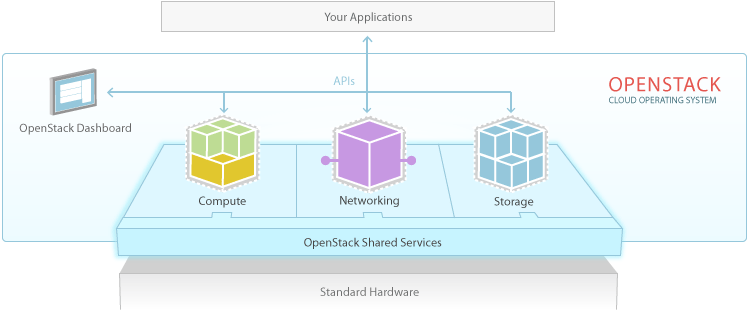
\includegraphics[width=1.0\linewidth]{openstack}
  \caption{OpenStack software diagram}\label{fig:openstack}
\end{figure}

The technology behind OpenStack consists of a series of interrelated projects delivering various components for a cloud infrastructure solution. Each service provides an open API so that all of these resources can be managed through a dashboard that gives administrators control while empowering users to provision resources through a web interface, a command-line client, or software development kits that support the API.

OpenStack is designed for horizontal scalability, so the user can easily add new compute, network, and storage resources to grow their cloud over time. In addition to the pervasiveness of massive OpenStack public clouds, many organizations, such as PayPal, Intel, and Comcast, build large-scale private clouds. OpenStack offers much more than a typical software package because it lets the user to integrate a number of different technologies to construct a cloud. This approach provides great flexibility, but the number of options might be daunting at first.

OpenStack clouds are powered by various OpenStack projects.
The selection of the components in openstack depends on how will the user be using OpenStack:

\begin{figure}[H]
  \centering
  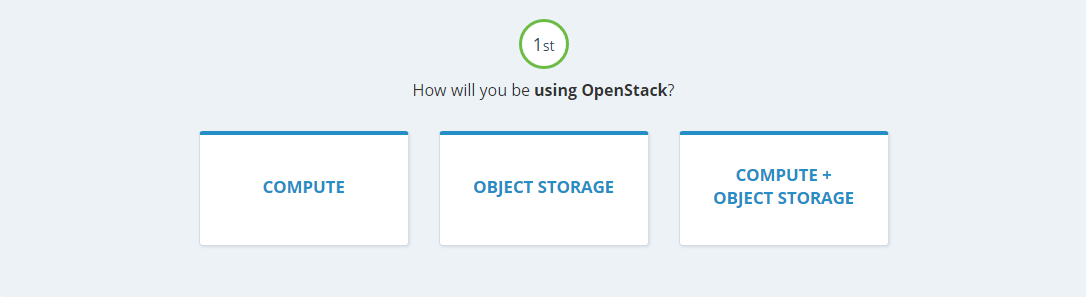
\includegraphics[width=1.0\linewidth]{Compute_ObjectStorage}
  \caption{Primary objective to decide the purpose of having an OpenStack Cloud}\label{fig:Compute_ObjectStorage}
\end{figure}

It actually specifies if the usage of OpenStack is, only with Compute - which defines the management of virtual machines on cloud, or only with Object Storage - which defines the allocation of end user based storage space on cloud, or the mix of both of Compute and Object Storage. Based on the objective of setting up the cloud, the core components can be selected as per the need from the wide range of available components.

\section{Motivation}\label{sec:motivation}

%\hint{Keep Scrolling!}\blindtext[1]
\comment{%
  \begin{itemize}
    \item The primary motivation the document is filled with huge amounts of blindtext, showing all the fancy stuff of \LaTeX{} and this template
    \item Go on scrolling though the document to find all the bells and wistles
    \item remove it, fill with your knowledge
    \item adapt the structure to your needs
  \end{itemize}
}
\blindlist{itemize}[3]
\blindtext[1]

\section{Ziel der Arbeit}\label{sec:ziel}

\blindtext[1]

\begin{figure}[htpb]
  \centering
  
\includegraphics[width=0.3\linewidth]{BildTBD}
  \caption{Hier könnte ein Bild stehen}\label{fig:bildtbd}
\end{figure}

Auch zeigt \cref{fig:bildtbd}, dass es genau so ist. Man könnte das auch mit einer \gls{gls:app}
realisieren. \missing{Quelle des Bildes noch ergänzen.}

\section{Struktur der Arbeit}\label{sec:struktur}

Die Arbeit gliedert sich wie folgt. \Cref{ch:grundlagen} erläutert wesentliche Grundlagen. Die theoretischen
Überlegungen zur Arbeit werden in \cref{ch:theorie} dargestellt. Die vorgenommene Entwicklung ist in \cref{ch:impl}
wiedergegeben.  \Cref{ch:Conclusion} fasst die Ergebnisse der Arbeit noch einmal zusammen und gibt einen Ausblick auf
zukünftige Entwicklungen.


% vim: ts=2:sw=2:sts=2:expandtab:wrapmargin=2:tw=120


	% !TEX root       = ./type_name.tex
% !TEX program    = pdflatex
% !TEX encoding   = utf-8
% !TeX spellcheck = en_GB
%=======================================================================

\chapter{Introduction}\label{ch:introduction}
\sffamily{}
The penetration of mobile internet users has increased many fold from a few thousands to millions over a short span of time. Due to the increasing demand for data among subscribers, mobile operators are pushed to go beyond boundaries to provide efficient and reliable data service to their customers. Although, the existing network services such as UMTS and LTE can handle larger data capacity, their coverage is not always sufficient in crowded places such as office buildings, convention centers, shopping malls etc. There is an urgent need to find a solution on how to offload the mobile data traffic over to other radio standards.

In such case, WLAN is an existing radio standard that has already been deployed in large numbers and has been supported by millions of devices lately. One unique advantage of using WLAN over other radio standards would be its license free usage of its radio frequency for commercial purposes. This WLAN standard, when deployed in a controlled manner can support data traffic routed from the mobile services. The IEEE 802.11 WLAN has already been widely used for commercial enterprises ranging from office networks, shopping malls to educational institutions etc. The deployment rages from a few dozens to hundreds of access points (APs), which serve many users through multitude of devices ranging from mobile devices, laptops to printers and other connected hardware. These networks also provide varied set of services that includes authentication, authorization and accounting (AAA), dynamic channel reconfiguration, interference management, security such as intrusion detection and prevention and providing quality of service. 

These enterprise WLAN AP’s are usually centrally managed through a controller. The task now is to find a solution to seamlessly direct traffic between LTE and WLAN. The research project BIC-IRAP (Business Indoor Coverage Integrated Radio Access Point) is currently aimed at providing a solution for the seamless coupling between LTE and WLAN.

The growing adoption of Software Defined Networking in the recent years has given rise to providing unique solutions without depending too much on hardware. The advantage of using SDN is that, it separates the network control pane from the physical network topology and uses software control flow to define how traffic is forwarded in the network. For example, the routing table and the flow control of a switch can be easily controlled remotely through a software controller.  The capabilities of SDN is possible due to the use of OpenFlow protocol which is a standardized protocol that is used by the SDN based controller to manipulate the flow tables of network switches. This provides more flexibility to programmatically control the behavior of network switches by building network applications that talk to the network controller. Any OpenFlow enabled switch from any vendor provides a common interface to be manipulated via a controller, thus providing flexibility and simplified network management.

%\comment{
%The cloud is a big deal for given reasons:
%\begin{itemize}
%	\item It does not need any effort on the consumer or the end user's part to maintain or manage it.
%	\item Any authenticated user can access the cloud-based applications and services from anywhere. All that the user needs is a device with an Internet connection.
%	\item It is effectively infinite in size, so that the consumer or the end user doesn't need to worry about it running out of capacity.
%	\item The resources can be scaled up or down quickly and easily to meet the desired changing demands of the consumer.
%	\item The services offered in the cloud are metered services, so the end user pay only for what they use.
%\end{itemize}
%}

\section{Contribution}\label{sec:contribution}

This thesis provides a novel approach towards separating the data traffic between the different network providers within an access point. This is made possible through the simple, yet effective use of OpenFlow protocol that enables the development of different enterprise WLAN services as applications such as, using software defined network controllers. The performance benefits achieved though this system is possible without any changes to the existing 802.11 client. The proposed system is compatible with the existing enterprise WLAN security protocols like WPA2 enterprise.

\section{Results}\label{sec:Results}
The expected outcome of this thesis is to demonstrate a prototype system that runs an AP on an OpenFLow controlled switch. The AP also provides enterprise grade authentication system WPA2 enterprise alongside a RADIUS server, and host two separate networks. The separation of data traffic between the two networks will take place within the same AP and provide Hotspot 2.0 functionality.

\section{Research Context\cite{BIC:IRAP}}\label{sec:BIC-IRAP}
The research described in this thesis was done based on the BIC-IRAP project which is focused on combining the strengths of LTE and Wireless-LAN seamlessly. Through the integration of small and micro cells of LTE with WLAN in the BIC-IRAP system, the two radio technologies are available through a single dynamically configurable hardware configuration.

\section{Thesis Structure}\label{sec:Structure}
This thesis report is organized as follows, Chapter 2 describes the background for this thesis. Chapter 3 describes in detail about SDN and the different types in use today. Chapter 4 talks about the control and authentication mechanism such as the protocols and technologies used. Chapter 5 talks about the environment required to build the system such as the tools and software’s. Chapter 6 describes in detail how the application is developed, from conceptualization to coding in python. Chapter 7 shows how the system is being implemented. Chapter 8 presents the results obtained from the system after series of testing and enhancement. Chapter 9 concludes the thesis and describes further improvements and drawbacks of this method.
	% !TEX root       = ./type_name.tex
% !TEX program    = pdflatex
% !TEX encoding   = utf-8
% !TEX spellcheck = de_DE_frami
%=======================================================================

%\chapter{Introduction}\label{ch:einleitung}
\chapter{Background}\label{ch:Background}
\sffamily{}

This chapter discusses about some basic fundamentals required to understand this thesis. It includes an introduction to software defined networking, explains the 802.11 protocol, provides a brief introduction to Hotspot 2.0 and also about the BIC-IRAP project.

\section{Software Defined Networking \cite{SDN}}\label{sec:SDN}

SDN is nothing but the physical separation of the network control plane from the forwarding plane. The control plane consists of all the logic (or instructions) that the switch requires for correctly setting up a forwarding plane.

Traditionally, the vendor has the control over the instructions necessary for signaling since the devices run a proprietary firmware within the switch. This makes the devices non-interoperable with other vendors, thus hampering flexibility. Though most of these switches provide \gls{SNMP} based management solution via Command Line Interface (CLI), they still do not allow the introduction of custom control plane function or protocol into the switch. This makes experimenting with new protocols cumbersome. Software Defined Networking aims to alleviate these problems by making the switched forwarding plane to be easily accessible remotely and modifiable using the OpenFlow protocol. Any third-party software can take advantage of this open protocol to manage and orchestrate an entire network.

SDN architecture generally has three components or groups of functionality as shown in figure \ref{fig:sdn-architecture}.

\begin{itemize}
	\item \textbf{Application Layer:}  Consists of programs that communicate the behaviors and needed resources with the SDN controller via the application protocol interfaces (API’s). It can also build an abstracted view of the network by collecting information from the controller.
	\item \textbf{Control Layer:} This logical layer functions as a relay that sends the instructions or resources sent by the application layer to the networking components.
	\item \textbf{Infrastructure Layer:} This holds the SDN networking devices that control the forwarding and data processing capabilities of the network including the function to forward and process the data paths.
\end{itemize}

\begin{figure}
  \centering
  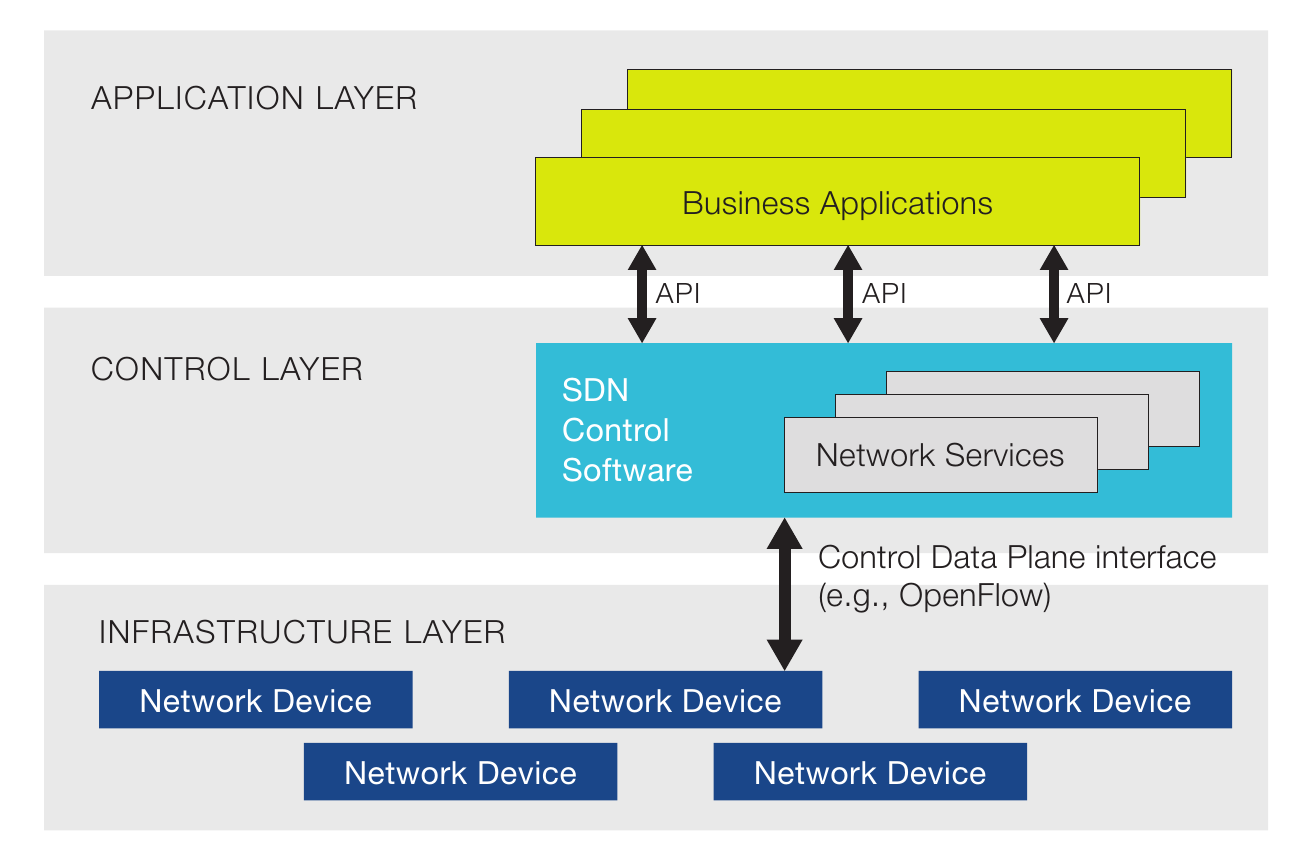
\includegraphics[width=1.0\linewidth]{sdn-architecture}
  \caption{SDN architecture diagram\cite{SDN:architecture}}
  \label{fig:sdn-architecture}
\end{figure}

\section{IEEE 802.11 MAC \cite{ieee2012802}}\label{sec:IEEE802.11}

The IEEE 802.11 \gls{MAC} \cite{ieee2012802} defines the protocol for stations to establish connections with each other and transmit data frames.
Medium access in 802.11 is performed by a distributed coordination function (DCF), which uses carrier sense multiple access with collision avoidance (CSMA/CA) to enable random medium access among all contending stations (STAs). Hence, it reduces the amount of collisions. Logically, the MAC is divided into two parts, an upper MAC, and a lower MAC. The upper MAC handles management frames, which include probe, authentication, association requests and their corresponding responses. The lower MAC handles control frames, which includes acknowledgment (ACK) frames, along with request-to-send (RTS) and clear-to-send (CTS) frames. The frames handled by the lower MAC have real-time constraints. For instance, ACK frame timeouts are within the order of micro-seconds. For this reason, control frames are handled and generated within hardware. Management frames, however, have softer time constraints, and can be handled in software locally (as is the case in Linux systems that use hostapd \cite{hostapd}), or remotely (as is the case when using a centralized WLAN controller \cite{RFC5412L97} ).

An 802.11 based wireless interface can operate under the following operating modes: STA (client), access point (AP), mesh, ad-hoc and item Monitor mode. The most common mode of operation is the infrastructure mode (which includes enterprise WLAN environments). In this mode of operation, clients connect to the AP using a series of message exchanges in a process called “association”. The decision on which AP to associate with is left entirely to the client. Clients learn about APs either passively through beacon frames that are periodically broadcasted by the access points, or actively by performing a probe scan. 

In a probe scan, clients first send out probe request frames over all channels. APs that receive these frames and are willing to accept a connection from a client respond with a probe response frame. All APs from which the client receives probe responses are candidates for the client to associate with. Next, the client sends an authentication frame, and waits for an authentication response from the AP. This is followed by the client sending an association request, and receiving an association response from the AP. If the network is operating in open authentication mode, the client is considered to be
associated at this point, and can now transmit data frames to be forwarded by the AP. If the AP is configured to use WPA, WPA2, or WPA2 Enterprise, the corresponding 802.1X \cite{hostapd} handshake is performed after the association phase before clients can forward data frames through the AP.


\section{Hotspot 2.0 \cite{Hotspot_2.0_Definition}} \label{Hotspot2.0}

It is a new wireless network standard that is designed to make connections to public Wi-Fi hotspots more easy and secure. They are already supported on many mobile devices running some popular operating systems such as Windows 10, Mac OS 10.9 or newer, Android 6.0 or newer, and iOS 7 or newer.

The main purpose of Hotspot 2.0 is to provide seamless mobility like cellular style “roaming” for Wi-Fi networks. The device will automatically connect to the available networks based on the network's partners on the home networks while roaming globally. This is made possible by using the latest 802.11u \cite{IEEE802.11u} protocol designed for the same purpose. The organization WIFI Alliance also calls this as Passpoint \cite{Passpoint}.
	% !TEX root       = ./type_name.tex
% !TEX program    = pdflatex
% !TEX encoding   = utf-8
% !TEX spellcheck = de_DE_frami
%=======================================================================

\chapter{Software Defined Networking}\label{ch:software_defined_networking}
\sffamily{}
The Open Network foundation, a non-profit organization, has been undertaking an extensive research for the past couple of years in designing and standardizing open network components such as OpenFlow, SDN etc. which, after being rolled out on to a variety of network devices and software’s from different vendors has been delivering substantial benefits to both enterprises and carriers include: \cite{What_is_SDN}

\begin{itemize}
	\item \textbf{Directly Programable:}Network directly programmable because the control functions are decoupled from forwarding functions, which enable the network to be programmatically configured by proprietary or open source automation tools.
	\item \textbf{Centralized Management:} Network intelligence is logically centralized in SDN controller software that maintains a global view of the network, which appears to applications and policy engines as a single, logical switch.
	\item \textbf{Reduce CapEx:} Software Defined Networking potentially limits the need to purchase purpose-built, ASIC-based networking hardware, and instead supports pay-as-you-grow models
	\item \textbf{Reduce OpEX:} SDN enables algorithmic control of the network of network elements (such as hardware or software switches/routers that are increasingly programmable, making it easier to design, deploy, manage, and scale networks. The ability to automate provisioning and orchestration optimizes service availability and reliability by reducing overall management time and the chance for human error.
	\item \textbf{Deliver Agility and Flexibility:} Software Defined Networking helps organizations rapidly deploy new applications, services, and infrastructure to quickly meet changing business goals and objectives.
	\item \textbf{Enable Innovation:} SDN enables organizations to create new types of applications, services, and business models that can offer new revenue streams and more value from the network.
	
\end{itemize}
\section{Existing SDN Controllers}\label{existing_sdn_controllers}
For this Master thesis, a few available SDN controllers are first studied for its functionality that can be manipulated for data path segregation. A brief overview on each controller is discussed in the following sections.
\subsection{Ryu Controller \cite{RYU_Switching_Hub}}\label{ryu_controller}
Ryu is a component-based software defined networking framework. It provides software components with well-defined API that make it easy to create new network management and control applications. The component that is of particular interest for this master thesis is the switching hub by using OpenFlow.

Switching hubs have a variety of functions, some of which are discussed below.
\begin{itemize}
	\item Learns the MAC address of the host connected to a port and retains it in the MAC address table.
	\item When receiving, packets addressed to a host already learned, transfers them to the port connected to the host.
	\item When receiving, packets addressed to an unknown host, performs flooding.
\end{itemize}

The main reason to choose RYU over other controllers is due to its customizability and easy to create core applications using Python. RYU allows users to modify core functions or use these functions to create custom applications that suits specific needs, in this case, it was used to create a switching application that can segregate users within the OpenVswitch, instead of being controlled each time by the controller.

The software components provided by RYU with well-defined Application Programming Interface (API’s), makes it easy for developers to create custom network management or control applications. The existing components can be quickly and easily modified or implement a custom component so that the underlying network can meet the changing demands of the application. RYU is designed to increase the agility of network by being more easily manageable and adapt how traffic is handled.

\begin{figure}[H]
	  \centering
	  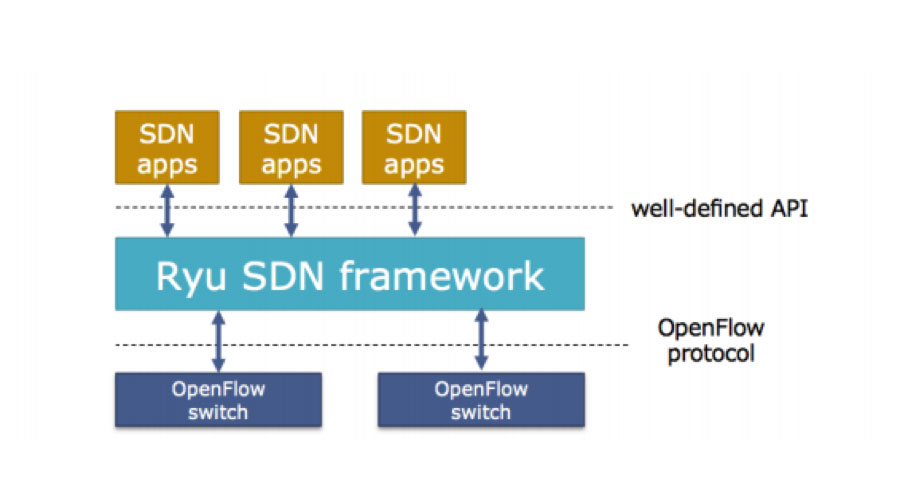
\includegraphics[width=1.0\linewidth]{ryu-controller-sdn-framework}
	  \caption{RYU SDN Controller Framework \cite{ryu_framewrk_png}} \label{fig:ryu-controller-sdn-framework}
	  \vspace{-10pt}
\end{figure}

RYU Controller is supported by NTT of Japan and has a strong open source RYU community that maintain and manage the code which is hosted at GitHub. OpenStack also supports deployment of RYU as network controller in its cloud operating systems.
\subsection{Floodlight Controller \cite{Floodlight_defn}} \label{Floodlight_Controller}

It is yet another open source SDN controller similar to RYU. The benefit of using this controller is the ability to easily develop applications using Java, which is widely used for high level programming by developers and to adapt the software as per requirement. Flood Light offers Representational state transfer application program interface (REST API’s) which help developers to easily program interfaces with the product.

Floodlight is used to run as the network backend for OpenStack. When used with the Neutron plugin with OpenStack, the Floodlight controller functions as a network-as-a-service model with the help of REST API offered by Floodlight. The following diagram below shows the architecture of Floodlight controller.

\begin{figure}[H]
	\centering
	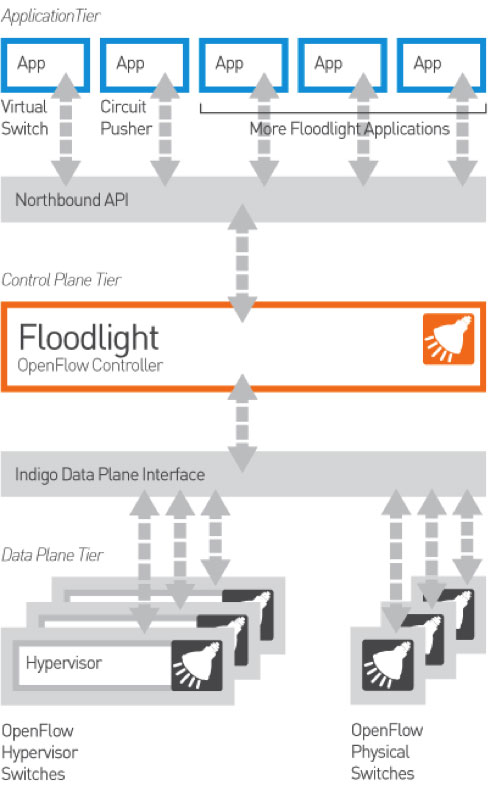
\includegraphics[width=\textwidth, height=\textheight]{floodlight-open-sdn-controller-diagram}
	\caption{Floodlight Controller architecture \cite{Floodlight_arch}} \label{fig:Floodlight_arch}
	\vspace{-10pt}
\end{figure}

\subsection{OpenDaylight} \label{Opendaylight}
OpenDaylight controller is based on JVM, similar to Floodlight, which was a derivative of OpenDaylight that can be deployed on any systems that supports Java. OpenDaylight controller uses the following tools as its framework:

\begin{itemize}
	\item \textbf{Maven:} OpenDaylight uses Maven, which uses Project Object Model to script the dependencies between the bundles for easier build automation.
	\item \textbf{OSGi:} It works as the back-end for OpenDaylight as it loads bundles dynamically and packages JAR files and binding them together for exchange of information.
	\item \textbf{JAVA interfaces:} They are used for event listening, specifications, and forming patterns. 
	\item \textbf{REST APIs:} These are the northbound APIs that manage the topology, flow program, host tracking, static routing and so on.
	
\end{itemize}

The following figure shows the framework of OpenDaylight with the above tools mentioned:

\begin{figure}[H]
	\centering
	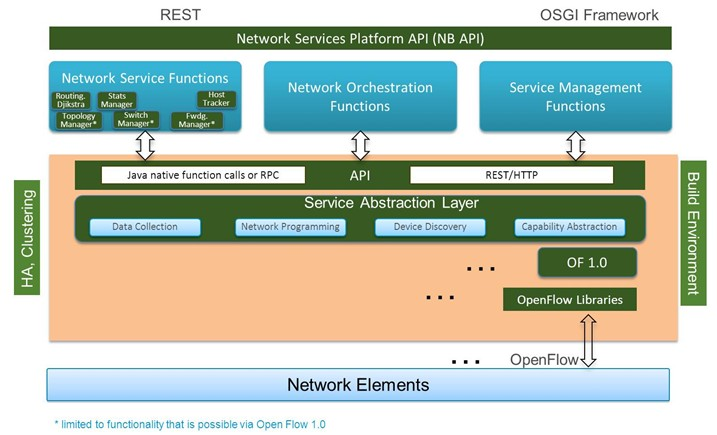
\includegraphics[width=1.0\linewidth]{Architectural_Framework}
	\caption{OpenDaylight Architecture Framework \cite{OpenDaylight_framework}} \label{fig:OpenDaylight_framework}
	\vspace{-10pt}
\end{figure}

\section{Applications of SDN} \label{SDN_applications}

Many research efforts has been done till now in writing SDN applications. Jose et. al. \cite{jose2011online} propose using commodity OpenFlow enabled switches for traffic measurement. The authors propose a framework where a collection of rules are installed on OpenFlow switches, and having a controller track the corresponding flow match counters. The controller can then draw inferences from the counters and dynamically tune the rules as required in order to identify different traffic aggregates.

Resonance \cite{Nayak:2009:RDA:1592681.1592684} is another application uses programmable switches to enforce access control in the network. The authors try to prove that today’s enterprise networks rely on different combinations of middle boxes, intrusion detection systems, and network configurations in order to enforce access control policies, whilst placing a burden on end-hosts in the system to remain patched and secure. The proposed system uses an SDN approach comprising programmable switches and a controller, which together implement a network monitoring framework, a policy specification framework, and the ability to trigger specific actions at the switch level.

OpenSAFE \cite{ballard2010extensible} is a framework that enables network monitoring using OpenFlow. It addresses the problem of routing traffic for network analysis in a reliable manner without affecting normal traffic. 

Hedera \cite{al2010hedera} is an adaptive flow scheduling system for data center networks. The premise for Hedera is that existing IP multipathing techniques used in data centers usually rely on per-flow static hashing, which can lead to under-utilisation of some network paths over time due to hash collisions. The system works by detecting large flows at the edge switches of a data center, and using placement algorithms to find good paths for the flows in the network. Experiments performed using simulations indicate significant improvements over static load balancing techniques. 

In the paper \textit{OpenFlow based server load balancing gone wild} \cite{wang2011openflow}, the authors address the problem of server load balancing using OpenFlow switches. The number of flow entries that can be saved on an OpenFlow switch is much less than the number of unique flows that a switch might need to handle in data center workloads. Thus, micro flow management using per-flow rules is not practical for performing distributing flows between different servers using a switch. The authors thus take advantage of OpenFlow’s wildcard based rules capability, and propose algorithms to compute concise wildcard rules that achieve a specific distribution of traffic.

These are some of the applications that have been written for SDN controllers but none of them address the challenge to dynamically redirect packets in real time, based on different clients and their credentials used for authentication. This thesis proposed to build one such application that can segregate packets coming from different clients in such a way that there is no possible connection between multiple clients associated within the same access point.

\section{Open vSwitch \cite{OpenVswitch_design}} \label{OpenvSwitch}
It is a production quality multilayer virtual switch, designed to enable massive automation through programmatic extension. It also supports standard management interfaces and protocols such as NetFlow, sFlow, CLI, port mirroring, VLAN’s, LACP etc. In addition to this, it is also designed to support distribution across multiple physical servers similar to VMWare’s vNetwork distributed vswitch. Open vSwitch was developed by the Linux foundation and is licensed under Apache 2.0.

The virtual switch is a software layer that resides in a server that is hosting virtual machines. VM’s and also now, containers such as Docker have logical and virtual Ethernet ports. These logical ports connect to a virtual switch. The diagram below shows the features of an Open vSwitch. \cite{WhatisOVS}
\begin{figure}[H]
	\centering
	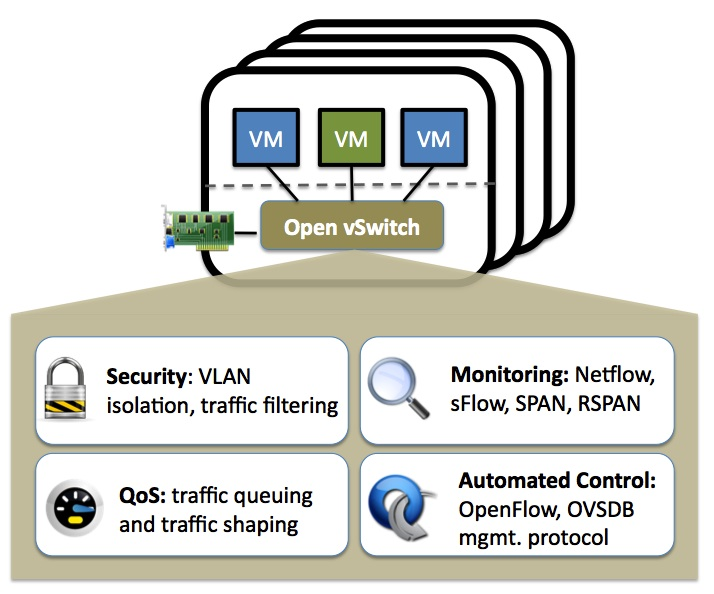
\includegraphics[width=1.0\linewidth]{ovs_schema}
	\caption{Open vSwitch features \cite{ovs_features}} \label{fig:OVS_Features}
	\vspace{-10pt}
\end{figure}

From the management and control perspective, Open vSwitch leverages on the OpenFlow and the Open vSwitch Database (OVSDB) management protocol, which means it can work as both a soft switch running within the hypervisor and as the control stack for switching operations on the physical switches. Other ways in which OVS is used in Software Defined Networking include:

\begin{itemize}
	\item SDN’s deployed in data centers use OVS because it connects all the virtual machines (VMs) within a hypervisor instance on a sever.
	\item It is the ingress point in overlay networks running on top of the physical networks in the data center and it is the first point of entry for all the VM’s sending traffic to the network.
	\item In datacenter SDN deployments, using OVS for virtual networking is considered the core element since its main use case is a multi-tenant network virtualization.
	\item In some service chaining use cases, OVS is sometimes used to direct traffic between network functions.
	
\end{itemize}

Open vSwitch is designed in such a way that it is meant to be managed and controlled by a third-party controllers and managers. OVS can also directly work with OpenStack using a plugin or directly from an SDN controller, such as OpenDaylight. It is also possible to deploy OVS on all servers in an environment and let it operate with the MAC learning functionality. 
	%% !TEX root       = ./type_name.tex
% !TEX program    = pdflatex
% !TEX encoding   = utf-8
% !TEX spellcheck = de_DE_frami
%=======================================================================

\chapter{Installation and Configuration of OpenStack}\label{ch:installationofopenstack}

The OpenStack consists of several key service projects which needs to be installed seperately.
These projects work together depending on the user's cloud needs.
The projects include Compute, Identity Service, Networking, Image Service, Block Storage, Object Storage, Telemetry, Orchestration, and Database.
Any services can be installed seperately and configure them stand-alone or as connected entities.

The Liberty version of OpenStack has been installed for the cloud test setup which has been documented in this thesis.
The OpenStack installation guide can also be found at \href{http://docs.openstack.org/liberty/install-guide-ubuntu/} {OpenStack Installation Guide for Ubuntu}.

The OpenStack project is an open source cloud computing platform that supports all types of cloud environments.
The project aims for simple implementation, massive scalability, and a rich set of features.
Cloud computing experts from around the world contribute to the project.

OpenStack provides an Infrastructure-as-a-Service (IaaS) solution through a variety of complemental services.
Each service offers an application programming interface (API) that facilitates this integration.


%\blindtext[1]

\section{Minimum hardware requirements for the compute purpose of the cloud}\label{sec:hardwarerequirements}
It requires at the least two nodes(hosts) to set up the OpenStack and launch a virtual machine or instance.
Optional services such as Block Storage and Object Storage require additional nodes.

The hardware architecture explained is the minimal hardware requirements for each type of node.
The figure \ref{fig:hwreqs} gives a general idea about the required nodes and optional nodes to start with an OpenStack for compute.

\begin{figure}[H]
  \centering
  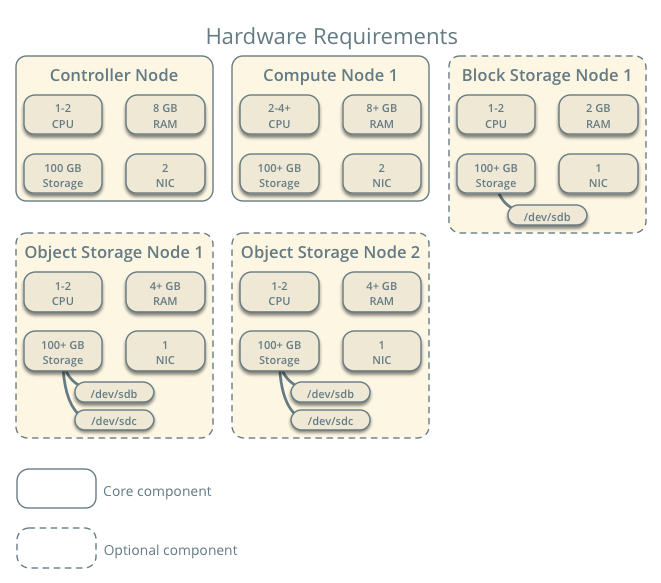
\includegraphics[width=1.0\linewidth]{hwreqs}
  \caption{Minimum hardware requirements to set up the OpenStack test bed\cite{OpenStack:hwreqs}}\label{fig:hwreqs}
  \vspace{-10pt}
\end{figure}


\subsection{Controller}\label{ssec:hwcontroller}
The \verb|controller| node runs the Identity service, Image service, management portions of Compute, management portion of Networking, various Networking agents, and the dashboard. It also includes supporting services such as an SQL database, message queue, and Network Time Protocol.

Optionally, the \verb|controller| node runs portions of Block Storage, Object Storage, Orchestration, and Telemetry services.

The \verb|controller| node requires a minimum of two network interfaces, 8 GB of RAM, 100 GB of storage space.

\subsection{Compute}\label{ssec:hwCompute}
The \verb|compute| node runs the hypervisor portion of Compute that operates instances.
By default, Compute uses the KVM hypervisor.
The \verb|compute| node also runs a Networking service agent that connects instances to virtual networks and provides firewalling services to instances via security groups.

You can deploy more than one \verb|compute| node.
Each node requires a minimum of two network interfaces,
more than 8 GB of RAM,
more than 100 GB of storage space and more than 2 CPU cores.

\subsection{Block Storage}\label{ssec:hwblockstorage}
This is an optional implementation and has not been set up for the test bed for this thesis.
The optional Block Storage node contains the disks that the Block Storage service provisions for instances.

You can deploy more than one block storage node.
Each node requires a minimum of one network interface.

\subsection{Object Storage}\label{ssec:hwobjectstorage}
This is also an optional implementation and has not been set up for the test bed for this thesis.
The optional Object Storage node contain the disks that the Object Storage service uses for storing accounts, containers, and objects.

This service requires two nodes.
Each node requires a minimum of one network interface.
You can deploy more than two object storage nodes.

\section{Networking Options}\label{sec:Networkingoptions}
OpenStack provides two diferent networking options:
\begin{itemize}
	\item Networking Option 1: Provider networks
	\\The provider networks option deploys the OpenStack Networking service in the simplest way possible with primarily layer-2 (bridging/switching) services and VLAN segmentation of networks.
	Essentially, it bridges virtual networks to physical networks and relies on physical network infrastructure for layer-3 (routing) services.
	Additionally, a DHCP service provides IP address information to instances.

	\item Networking Option 2: Self-service networks
	\\The self-service networks option augments the provider networks option with layer-3 (routing) services that enable self-service networks using overlay segmentation methods such as VXLAN.
	Essentially, it routes virtual networks to physical networks using NAT.
	Additionally, this option provides the foundation for advanced services such as LBaaS and FWaaS.
\end{itemize}

Considering the network options, the networking option 2 of self service networks have been implemented for the test bed.

%Weiterführende Informationen zu diesem Thema bietet~\cite{Herrmann2004}. In dem Buch werden auch Details zu \acp{ic}
%dargestellt.
%\blindtext[2]
%\blindenumerate{}
%\blindtext[2]

\section{Configuration of Services and config files}\label{sec:configurationofopenstack}

For the test bed of this thesis, there is one \verb|controller| node and four \verb|compute| nodes which have been configured.
All the nodes have been installed with the \verb|Ubuntu 14.04| \verb|LTS| Operating system.
For the purpose of having the GUI, the desktop version of the Operating system has been set up on each node.

This thesis does not explain the installation in detail as it is already available in \href{http://docs.openstack.org/liberty/install-guide-ubuntu/} {OpenStack Installation Guide for Ubuntu}.
This thesis covers the basics of the topics which were covered during the setup of the test bed are documented. And also, the problems that were faced due to some of the missing configurations as they were not mentioned in the \href{http://docs.openstack.org/liberty/install-guide-ubuntu/} {OpenStack Installation Guide for Ubuntu} are documented in this section.

To keep the configuration of the testbed simple, the password used for convenience on all the host machines and all the OpenStack services is \verb|user|.


\subsection{Host networking}\label{ssec:Hostnetworkingarchitecture}

\begin{figure}[H]
  \centering
  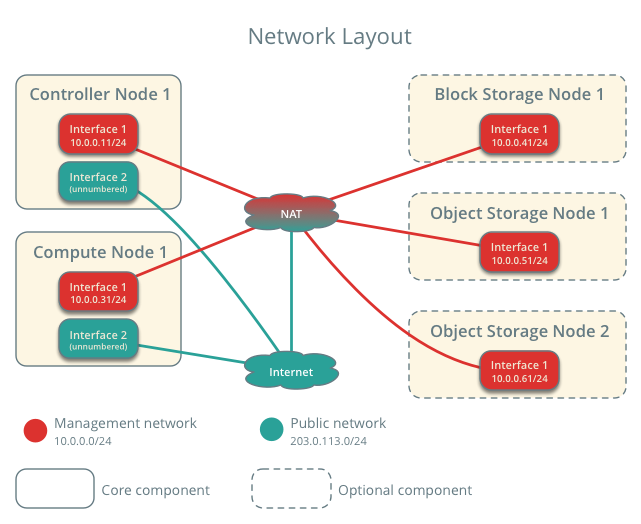
\includegraphics[width=1.0\linewidth]{networklayout}
  \caption{Network layout among all the host machines\cite{OpenStack:networklayout}}\label{fig:networklayout}
\end{figure}
The figure \ref{fig:networklayout} shows how the connections are established between all the node machines.
A private management network and a public network provided with internet connection are set up for the \verb|controller| and \verb|compute| nodes.
The management network's IP for the network interface of \verb|controller| node is set to static IP of \verb|10.0.0.11|.
Similarly, the management network's IP for one of the network interfaces on the five of the \verb|compute| nodes have the static IPs ranging from \verb|10.0.0.31| to \verb|10.0.0.35|.

In this thesis, the storage nodes have not been implemented.

For the testbed setup, one \verb|controller| node and five computes nodes have been set up.


\subsection{Network Time Protocol (NTP)}\label{ssec:NetworkTimeProtocol_NTP}
The Chrony application is installed on all the nodes to synchronise the time on all the installed nodes.
The \verb|controller| node is set to synchronise with the network time server provided by "TU-Chemnitz" given by the server host name as \verb|ntphost1.hrz.| \verb|tu-chemnitz.de|.
The other \verb|compute| nodes are set to have the synchronised time with the \verb|controller| node by setting the \verb|controller| node as network time server.

\subsection{OpenStack packages}\label{ssec:OpenStackpackages}
OpenStack packages are installed on all the nodes by enabling the OpenStack repository and installing all required basic packages.

The MariaDB SQL database server is installed on the \verb|controller| node to store the information related to OpenStack services for authentication and other related activities.
The MongoDB NoSQL database is installed on the \verb|controller| for the purpose of Telemetry service (Ceilometer).

OpenStack uses the message queue to co-ordinate operations and services among the installed services.
The RabbitMQ server is installed on the \verb|controller| node to provide the message queue service among the services.


\subsection{Add the Identity service}\label{ssec:AddtheIdentityservice}
The OpenStack Identity service provides a single point of integration for managing authentication, authorization, and service catalog services.
Other OpenStack services use the Identity service as a common unified API.

When an OpenStack service receives a request from a user, it checks with the Identity service whether the user is authorized to make the request.

In the setup, the Identity service has been installed on the \verb|controller|.

The keystone service entity and API endpoints are created to enable and access the Identity service by internal service calls and from the external requests using the REST based API.
The public, the internal and the admin endpoints are created to access the Identity service.
These three endpoints are created across all further services installed.

Each service that you add to your OpenStack environment requires one or more service entities and three API endpoint variants in the Identity service.

While configuring the endpoints for the Identity service, the \verb|region| is set to \verb|TUChem|-\verb|nitz|.
For example:
\begin{lstlisting}[frame=single]
$ openstack endpoint create --region TUChemnitz identity public http://controller:5000/v2.0
\end{lstlisting}

\comment{A point to remember is, do not duplicate the given endpoints for a given region.
This has caused the issue with failure of the service.}

Create the projects, users, and roles in the Identity service to access the services for \verb|compute| users for user specific projects based on the access permissions.

The test bed has two projects (admin, demo) for test, 3 diferent users (admin, demo, service) to different access permissions defined by two roles (admin, user).

\subsection{Add the Image service}\label{ssec:AddtheImageservice}
The OpenStack Image service is central to Infrastructure-as-a-Service (IaaS) as shown in figure \ref{fig:openstack_architecture}.
It accepts API requests for disk or server images, and image metadata from end users or OpenStack Compute components.
It also supports the storage of disk or server images on various repository types, including OpenStack Object Storage.

The SQL database is used to store the metadata information of the operating system image or the server image or the disk storage.
There are templates available of specified requirements to create a virtual machine.
These templates are called as flavors in OpenStack.
The details of requirements to boot a virtual machine is defined in these flavors.
For example, the hard disk capacity, the RAM capacity, the number of virtual cores, which would be required to satisfy the minimum requirements criteria of the desired operating system or to build a robust compute machine with a higher configurations a template is created to give as an input to the scheduler to create a virtual machine.

This service is installed on \verb|controller| node.
The glance service entity and the API endpoints are created.
While configuring the endpoints for the Image service, the \verb|region| is set to \verb|TUChemnitz|.
For example:
\begin{lstlisting}[frame=single]
$ openstack endpoint create --region TUChemnitz image public http://controller:9292
\end{lstlisting}

The \verb|cirros-0.3.4-x86_64-disk.img| disk image was downloaded and added to the image service as a bootable image of Cirros operating system to create and boot virtual machines.


\subsection{Add the Compute service}\label{ssec:AddtheComputeservice}
OpenStack Compute is a major part of an Infrastructure-as-a-Service (IaaS) system.
The main modules are implemented in Python.

OpenStack Compute interacts with OpenStack Identity for authentication, OpenStack Image service for disk and server images, and OpenStack dashboard for the user and administrative interface. Image access is limited by projects, and by users; quotas are limited per project (the number of instances, for example). OpenStack Compute can scale horizontally on standard hardware, and download images to launch instances.

The nova service entity and the API endpoints are created.
While configuring the endpoints for the Compute service, the \verb|region| is set to \verb|TUChemnitz|.
For example:
\begin{lstlisting}[frame=single]
$ openstack endpoint create --region TUChemnitz compute public http://controller:8774/v2/%\(tenant_id\)s
\end{lstlisting}

RabbitMQ which is the installed message queue server is used to pass the communication messages between the nodes and the other services.
The MariaDB SQL database stores the build-time and run-time states of the whole cloud infrastructure like available instance, instances in use, available networks and different projects.

The OpenStack compute is installed with required packages on \verb|controller| node which are different than the \verb|compute| node.
The important compute services like \texttt{nova-scheduler, nova-conductor, nova-api, nova-cert, nova-novncproxy} and \texttt{python-novaclient} are installed on the \verb|controller| node.
The configuration of RabbitMQ message service needs some additional parameters that needs to be added in the \verb|/etc/nova/nova.conf| configuration file in the \verb|controller| node under the \verb|[oslo_messaging_rabbit]|.

\begin{lstlisting}[frame=single]
[oslo_messaging_rabbit]
rabbit_host = controller
rabbit_port = 5672 #define ports
rabbit_hosts = controller:5672
rabbit_userid = openstack
rabbit_password = user
rabbit_use_ssl = false
\end{lstlisting}

\comment{The compute service failed to function when the \texttt{rabbit\_port} was not defined in the configuration.}

The OpenStack compute is installed with the \verb|nova-compute| package on all the \verb|compute| nodes.
The configuration of RabbitMQ message service needs some additional parameters that needs to be added in the \verb|/etc/nova/nova.conf| configuration file in the \verb|compute| nodes under the \verb|[oslo_messaging_rabbit]|.
\\Please refer to Appendix \nameref{app:sec:rabbitmq_config} for the \verb|[oslo_messaging_rabbit]| configuration parameters.

%\begin{lstlisting}[frame=single]
%[oslo_messaging_rabbit]
%rabbit_host = controller
%rabbit_port = 5672 #define ports
%rabbit_hosts = controller:5672
%rabbit_userid = openstack
%rabbit_password = user
%rabbit_use_ssl = false
%\end{lstlisting}

In the \texttt{[DEFAULT]} section of the \verb|/etc/nova/nova.conf| file in \verb|compute| nodes, configure the \verb|my_ip| option with their respective management IP address of the compute nodes.

In the \texttt{[vnc]} section of the \verb|/etc/nova/nova.conf| file in \verb|compute| nodes, enable and configure remote console access by providing the public base url of the \verb|controller| node to make it accessible from any machine outside the management network.

\begin{lstlisting}[frame=single]
[vnc]
enabled = True
vncserver_listen = 0.0.0.0
vncserver_proxyclient_address = $my_ip
novncproxy_base_url = http://os-controller.etit.tu-chemnitz.de:6080/vnc_auto.html
\end{lstlisting}

Verify the operation of the Compute service by performing the commands as stated in the \href{http://docs.openstack.org/liberty/install-guide-ubuntu/} {OpenStack Installation Guide for Ubuntu}.

\subsection{Add the Networking service}\label{ssec:AddtheNetworkingservice}
This section explains about installation and configuration of the OpenStack Networking service (neutron) using the \verb|self-service networks| option.
OpenStack Networking (neutron) allows you to create and attach interface devices managed by other OpenStack services to networks.

OpenStack Networking (neutron) manages all networking facets for the Virtual Networking Infrastructure (VNI) and the access layer aspects of the Physical Networking Infrastructure (PNI) in any given OpenStack environment.
OpenStack Networking enables tenants to create advanced virtual network topologies which may include services such as a firewall, a load balancer, and a virtual private network (VPN).

Networking provides networks, subnets, and routers as object abstractions.

The neutron service entity and the API endpoints are created.
While configuring the endpoints for the Networking service, the \verb|region| is set to \verb|TUChemnitz|.
For example:
\begin{lstlisting}[frame=single]
$ openstack endpoint create --region TUChemnitz network public http://controller:9696
\end{lstlisting}
The Networking option 2: Self service networks is adapted for configuration of the test bed.

The required neutron networking components are installed on the \verb|controller| node.
The configuration of RabbitMQ message service needs some additional parameters that needs to be added in the \verb|/etc/neutron/neutron.conf| configuration file in the \verb|controller| node under the \verb|[oslo_messaging_rabbit]|.
\\Please refer to Appendix \nameref{app:sec:rabbitmq_config} for the \verb|[oslo_messaging_rabbit]| configuration parameters.

%\begin{lstlisting}[frame=single]
%[oslo_messaging_rabbit]
%rabbit_host = controller
%rabbit_port = 5672 #define ports
%rabbit_hosts = controller:5672
%rabbit_userid = openstack
%rabbit_password = user
%rabbit_use_ssl = false
%\end{lstlisting}

In the \verb|/etc/neutron/neutron.conf| configuration file of the controller, under the \verb|[nova]| section, the \verb|region_name| is set to \verb|TUChemnitz|.
\begin{lstlisting}[frame=single]
[nova]
...
region_name = TUChemnitz
\end{lstlisting}

In the \verb|/etc/neutron/metadata_agent.ini| file of the controller, under the \verb|[DEFAULT]| section, the \verb|auth_region| is set to \verb|TUChemnitz|.
The \verb|metadata_proxy_shared_-| \verb|secret| is set to \verb|user| which will be used in \verb|/etc/nova/nova.conf| configuration file.
\begin{lstlisting}[frame=single]
[DEFAULT]
...
auth_region = TUChemnitz
...
metadata_proxy_shared_secret = user
\end{lstlisting}

Edit the \verb|/etc/nova/nova.conf| configuration file to set the \verb|metadata_proxy_share|-\verb|d_secret| with the value of \verb|user|.
\begin{lstlisting}[frame=single]
[neutron]
...
region_name = TUChemnitz
...
metadata_proxy_shared_secret = user
\end{lstlisting}

Once the \verb|controller| node has been set up, the common Networking components are installed on each of the \verb|compute| nodes.
The configuration of RabbitMQ message service needs some additional parameters that needs to be added in the \verb|/etc/neutron/n|-\verb|eutron.conf| configuration file in each of the \verb|compute| node under the \verb|[oslo_messag|-\verb|ing_rabbit]|.
\\Please refer to Appendix \nameref{app:sec:rabbitmq_config} for the \verb|[oslo_messaging_rabbit]| configuration parameters.

%\begin{lstlisting}[frame=single]
%[oslo_messaging_rabbit]
%rabbit_host = controller
%rabbit_port = 5672 #define ports
%rabbit_hosts = controller:5672
%rabbit_userid = openstack
%rabbit_password = user
%rabbit_use_ssl = false
%\end{lstlisting}

As the \textit{Networking option 2: Self service networks} was set up in \verb|controller| node, the Linux bridge agent, which builds layer-2 (bridging and switching) virtual networking infrastructure for instances including VXLAN tunnels for private networks and handles security groups, is configured on each \verb|compute| node.

As in \verb|controller| node, the \verb|compute| nodes are configured to use the networking service by editing the \verb|/etc/nova/nova.conf| configuration file on each \verb|compute| node.
\begin{lstlisting}[frame=single]
[neutron]
...
region_name = TUChemnitz
\end{lstlisting}

The configuration of networking service is verified to have all the services of networking to be active.

\subsection{Add the dashboard}\label{ssec:Addthedashboard}
The OpenStack Dashboard, also known as horizon is a web interface that enables cloud administrators and users to manage various OpenStack resources and services.

The Dashboard enables web-based interactions with the OpenStack Compute cloud controller through the OpenStack APIs.

Horizon enables you to customize the brand of the dashboard.

The dashboard relies on functional core services including identity, image, compute, and neutron.
The dashboard is installed on the \verb|controller| node.

The figure \ref{fig:dashboard_login} shows the login screen for the OpenStack dashboard.

\begin{figure}[H]
  \centering
  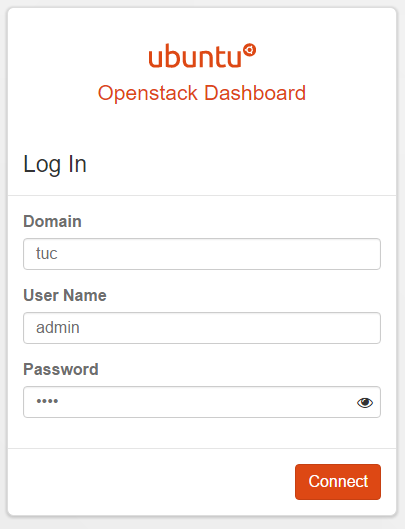
\includegraphics[width=0.7\linewidth]{dashboard_login}
  \caption{Login screen for the dashboard}\label{fig:dashboard_login}
\end{figure}
The dashboard can be accessed by using the web browser at: \\\verb|http://os-controller.etit.tu-chemnitz.de/horizon|.

Provide the login credentials to authenticate the user against the Keystone to login into the Dashboard.\\

The login credentials are:
\\Domain: \verb|TUC|
\\User Name: \verb|admin| or \verb|demo|
\\Password: user

The figure \ref{fig:network_topology_dashboard_view} shows the pictorial representation of the network and the instances created on the OpenStack under the link \textit{Network Topology}.

\begin{figure}[H]
  \centering
  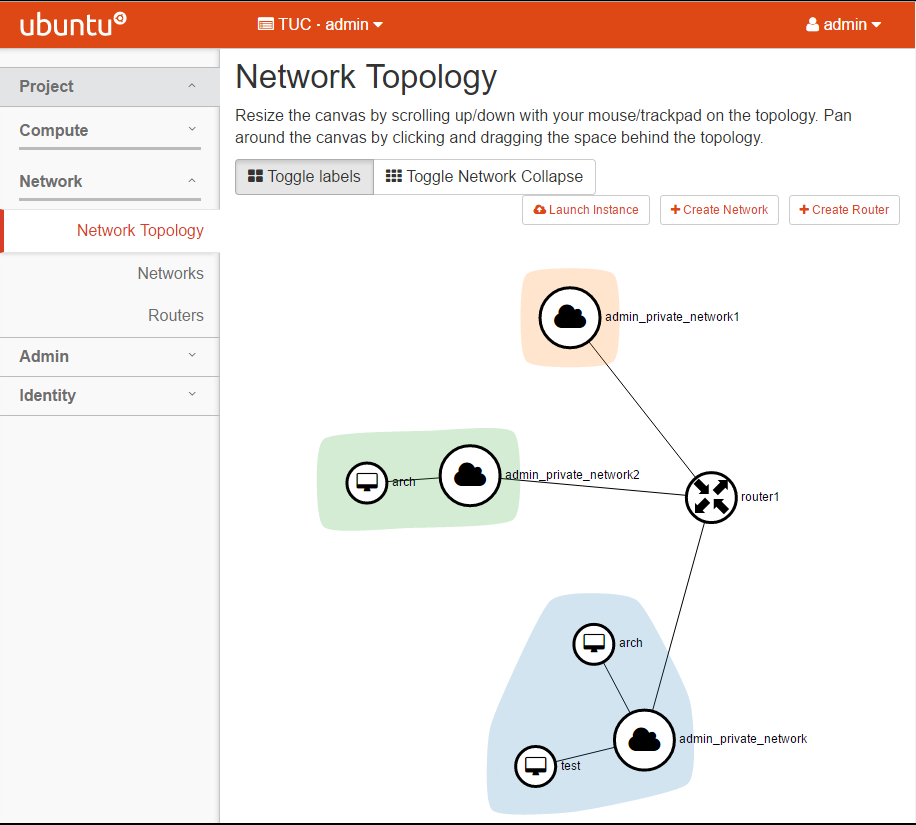
\includegraphics[width=1.0\linewidth]{network_topology_dashboard_view}
  \caption{The dashboard screen showing the diagrammatic representation of network topology}\label{fig:network_topology_dashboard_view}
\end{figure}

\subsection{Add the Telemetry service}\label{ssec:AddtheTelemetryservice}
The Object storage and Bloack storage services have not been deployed for the test bed.
The next service deployed is the OpenStack Telemetry service.

Telemetry service is deployed to have an analysis of metering data with respect to Compute and Image services.
Telemetry helps to efficiently poll the metering data related to OpenStack services.

Unlike other services, the Telemetry service uses a NoSQL database.
The MongoDB NoSQL server has been installed on the controller to be utilised by the Telemetry service.
The \verb|password| for the MongoDB is set to \verb|user|.

The ceilometer service entity and the API endpoints are created.
While configuring the endpoints for the Telemetry service, the \verb|region| is set to \verb|TUChemnitz|.
For example:
\begin{lstlisting}[frame=single]
$ openstack endpoint create --region TUChemnitz metering public http://controller:8777
\end{lstlisting}


The configuration of RabbitMQ message service needs some additional parameters that needs to be added in the \verb|/etc/ceilometer/ceilometer.conf| configuration file on the \verb|controller| node under the \verb|[oslo_messaging_rabbit]|.
\\Please refer to Appendix \nameref{app:sec:rabbitmq_config} for the \verb|[oslo_messaging_rabbit]| configuration parameters.
%\begin{lstlisting}[frame=single]
%[oslo_messaging_rabbit]
%rabbit_host = controller
%rabbit_port = 5672 #define ports
%rabbit_hosts = controller:5672
%rabbit_userid = openstack
%rabbit_password = user
%rabbit_use_ssl = false
%\end{lstlisting}

In the \verb|[service_credentials]| section, the \verb|os_region_name| is set as \verb|TUChemnitz|.
\begin{lstlisting}[frame=single]
[service_credentials]
...
os_region_name = TUChemnitz
\end{lstlisting}

Once the Telemetry service has been installed on \verb|controller|, it is configured to be consumed by Image service by editing the existing \verb|/etc/glance/glance-api.conf| and \verb|/etc/glance/glance-registry.conf| configuration files by adding the \\\verb|[oslo_messaging_rabbit]|.
\\Please refer to Appendix \nameref{app:sec:rabbitmq_config} for the \verb|[oslo_messaging_rabbit]| configuration parameters.

%\begin{lstlisting}[frame=single]
%[oslo_messaging_rabbit]
%rabbit_host = controller
%rabbit_port = 5672 #define ports
%rabbit_hosts = controller:5672
%rabbit_userid = openstack
%rabbit_password = user
%rabbit_use_ssl = false
%\end{lstlisting}

Once the OpenStack installation procedure with additional configuration as mentioned above is configured, the Telemetry is for Image service.

To enable the Telemetry service for Compute service, the ceilometer should be installed on each \verb|compute| node.
Once the Telemetry service has been installed on all the \verb|compute| nodes, it is configured to enable ceilometer by editing the \verb|/etc/ceilometer|-\verb|/ceilometer.conf| configuration file by adding the \verb|[oslo_messaging_rabbit]|.
Please refer to Appendix \nameref{app:sec:rabbitmq_config} for the \verb|[oslo_messaging_rabbit]| configuration parameters.

%\begin{lstlisting}[frame=single]
%[oslo_messaging_rabbit]
%rabbit_host = controller
%rabbit_port = 5672 #define ports
%rabbit_hosts = controller:5672
%rabbit_userid = openstack
%rabbit_password = user
%rabbit_use_ssl = false
%\end{lstlisting}

In the \verb|[service_credentials]| section, the \verb|os_region_name| is set as \verb|TUChemnitz|.
\begin{lstlisting}[frame=single]
[service_credentials]
...
os_region_name = TUChemnitz
\end{lstlisting}


\begin{figure}[H]
  \centering
  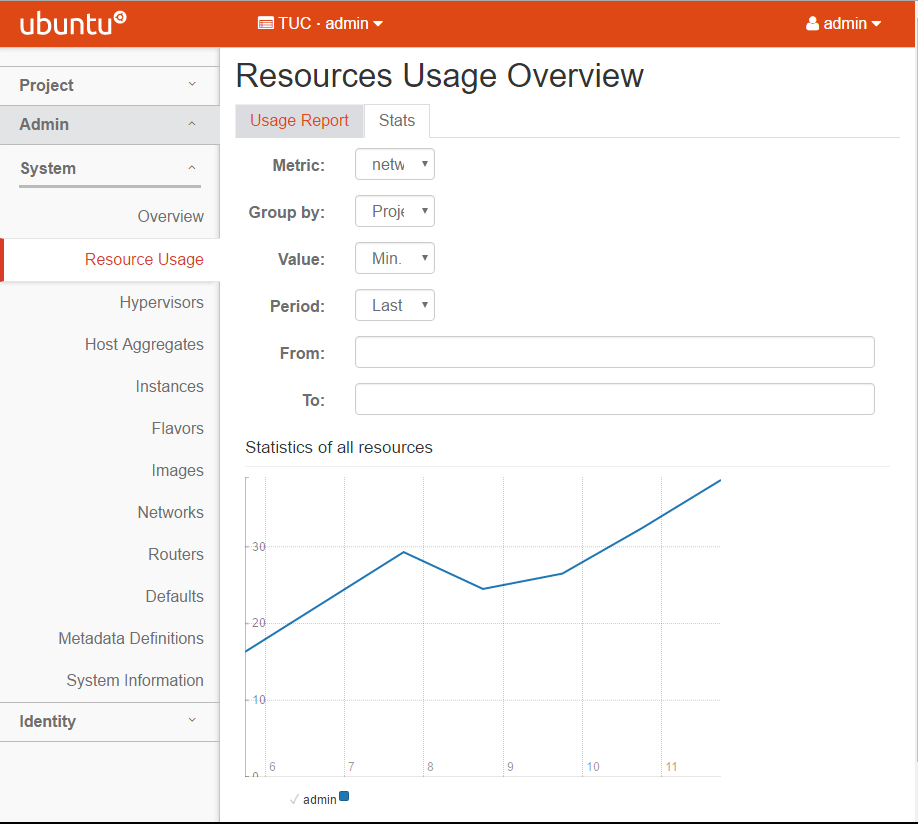
\includegraphics[width=1.0\linewidth]{telemetry_network_incoming_bytes}
  \caption{An example of the metering with the number of incoming bytes on a network for a virtual machine interface.}\label{fig:telemetry_network_incoming_bytes}
\end{figure}

All the above mentioned services have been installed and configured in the OpenStack test bed for this thesis.

%Das hier vorgestellte basiert auch dem Buch von~\cite{Heinkel2000}. Die Lösung kann auch mit einem \ac{fpga} sowie
%\ac{hw} und \ac{sw} entstehen.
%\blindtext[4]

%\subsection{Zweite Untergrundlage}\label{ssec:zweiteUGdl}

%\blindtext[1]
%\begin{table}[htpb]
%  \centering
%  \caption{Eine tolle Tabelle}\label{tab:ett}
%  \begin{tabular}{lcrl}
%  Links & Zentriert & Rechts & Links \\
%  \toprule
%  eins & zwei & drei & vier \\
%  eins & zwei & drei & vier \\
%  eins & zwei & drei & vier \\
%  \end{tabular}
%\end{table}

%Eine Tabelle benötigt auch eine Referenz, wie diese hier zu \ref{tab:ett}.
%\blindtext[1]

%\section{Zweite Grundlage}\label{sec:zweitegdl}

%\blindtext[2]

%\section{Dritte Grundlage}\label{sec:drittegdl}

%\blindtext[2]

% vim: ts=2:sw=2:sts=2:expandtab:wrapmargin=2:tw=120


	% !TEX root       = ./type_name.tex
% !TEX program    = pdflatex
% !TEX encoding   = utf-8
% !TEX spellcheck = de_DE_frami
% Please add the following required packages to your document preamble:
%\usepackage{booktabs}
%\usepackage{graphicx}
%\usepackage[table,xcdraw]{xcolor}
% If you use beamer only pass "xcolor=table" option, i.e. \documentclass[xcolor=table]{beamer}
%=======================================================================

\chapter{Control and Authentication Mechanism}\label{ch:control_and_authentication}
\sffamily{}

In this chapter, the softwares and protocols used for providing authentication and for controlling the access point is discussed. A brief introduction to OpenWrt and the protocols, OpenFlow and RADIUS is described in the flowing topics.
\section{OpenWrt \cite{WhatIsOpenWrt}} \label{OpenWrt}

OpenWrt is a Linux distribution that works like any other Linux distro designed for embedded devices. OpenWrt offers bult-in package manager that allows installing packages from its repository or manually build custom firmware file using custom-built package. The packages can contain many supported applications like an SSH server, VPN, traffic-shaping application, enterprise wireless solutions, BitTorrent client and even a hotspot manager.

OpenWrt is designed for power users who require customizability over the stock firmware provided by the manufacturer. There are many custom firmwares such as DD-WRT available for most popular routers. For this thesis, OpenWrt is chosen because of its flexibility and stability than most custom firmwares that are available for many hardware vendors.

OpenWrt has many features that can be mentioned but are out of scope for this thesis. A run-down version of the most relevant features are listed below that are related to this thesis.

\begin{itemize}
	\item \textbf{SSH server for terminal access:} Provides SSH server, which allows to connect directly to the routers terminal via SSH and remote configuration is also possible when the router is configured to connect with the internet. 
	\item \textbf{Capture and Analyse network Traffic:} Tcpdump tool is included in the build to analyze the packets that are traversing through the router. The tool can also be used to create packet logs that can be opened in packet analyzer tools such as Wireshark.
	\item \textbf{GUI Interface:} OpenWrt also includes a GUI interface for managing most of the routers configuration, the built in one is named as LuCi.
	\item \textbf{OpenvSwitch:} The virtual switch is also available as a package on OpenWrt repository that is used in this thesis to be installed in the router for creating a virtual switch within the router that can also work along with the physical switches present.
	\item \textbf{Wireless Utilities:} OpenWrt provides many different packages for managing wireless sockets in the router. For this thesis, Hostapd package is chosen because of its fully featured support for a wide range of authentication mechanisms such as IEEE 802.1x/WPA/EAP/RADIUS with EAP protocol. It can be configured in the file located at /etc/hostapd.conf in the routers folder.
	\item \textbf{Freeradius:} The open source RADIUS server is also available as a package for the OpenWrt build but is not used in the firmware for this thesis because of memory unavailability in the TP Link WDR-4300 router.
	\item \textbf{MySQL:} The is a fully featured MySql server. It is also available as a package that can be installed on the router but again could not be used in this thesis due to memory restrictions in the router.
	
\end{itemize}
The figure \ref{fig:OpenWrt_terminal} shows the SSH interface of OpenWrt terminal and the figure \ref{fig:OpenWrt_gui} shows the LuCi web interface.
\begin{figure}
	\centering
	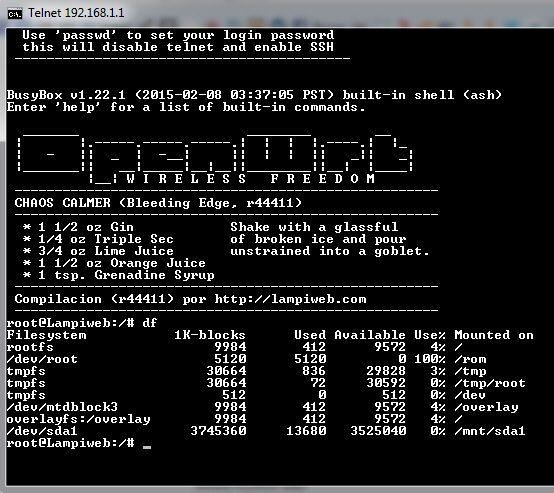
\includegraphics[width=1.0\linewidth]{openwrt4-terminal}
	\caption{OpenWrt Terminal View \cite{openwrt_terminal_img}} \label{fig:OpenWrt_terminal}
	\vspace{-10pt}
\end{figure}

\begin{figure}
	\centering
	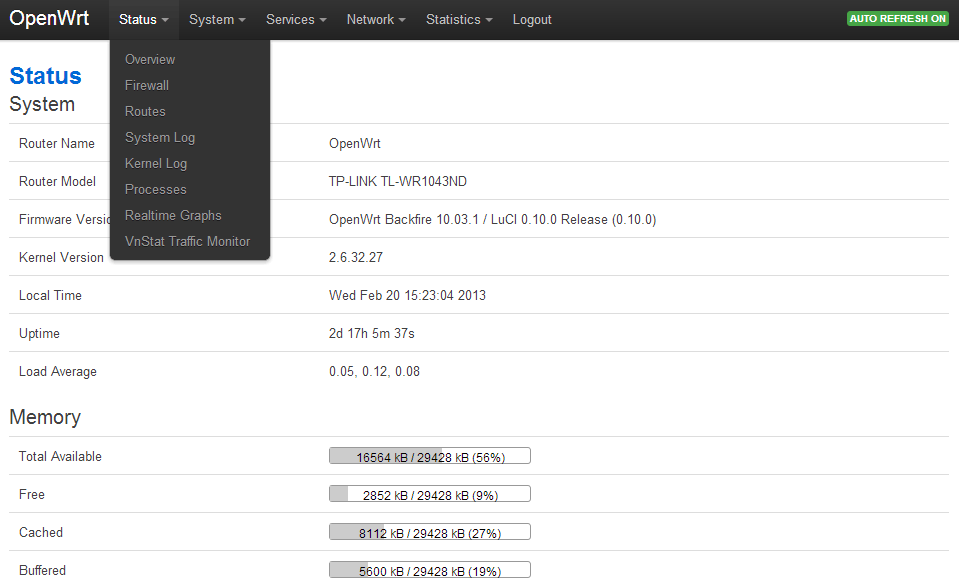
\includegraphics[width=1.0\linewidth]{bootstrap-luci-theme}
	\caption{OpenWrt GUI Interface \cite{openwrt_luci_img}} \label{fig:OpenWrt_gui}
	\vspace{-10pt}
\end{figure}
\section{Protocols} \label{protocols}
For this thesis, protocols such as OpenFlow, RADIUS and 802.1x security are used extensively and are discussed in detail below, explaining their use cases and features.
\subsection{OpenFlow \cite{WhatIsOpenFlow}} \label{OpenFlow}

It is a standard communication interface defined between the control and forwarding layers of the SDN architecture, allowing direct access for manipulating the forwarding plane of the network devices such as switches and routers, both physical and virtual (hypervisor based).

OpenFlow, along with SDN technologies have helped IT to manage and address the high-bandwidth, and dynamic nature of today’s applications. It also has helped adapt the network to ever-changing business needs, and significantly reduce the complexity in maintenance and operations. The successful deployment \cite{of_depl} of OpenFlow in large organizations such as Google \cite{of_google}, Géant of Switzerland,ToulX France etc. shows what can be achieved with OpenFlow and the extent to which its features can be utilized.

%Some of the best features of OpenFlow obtained from its successful deployments  is explained in the figure \ref{fig:OF_features}.
%
%\begin{figure}
%	\centering
%	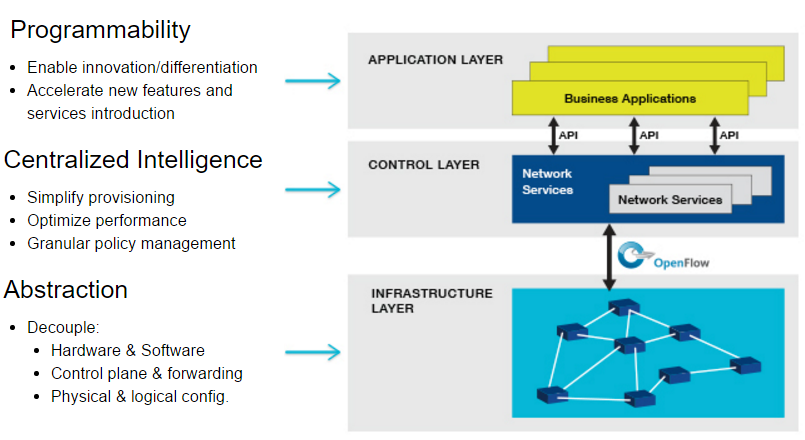
\includegraphics[width=1.0\linewidth]{of-features}
%	\caption{OpenFlow features \cite{openflow_features}} \label{fig:OF_features}
%	\vspace{-10pt}
%\end{figure}

\subsubsection{How does OpenFlow Work? \cite{OpenFlow_functionality}} \label{OpenFlow_Functionality}
In a traditional switch or a router, the packet forwarding and high level routing decisions occur on the same device. In an OpenFlow switch, the routing and forwarding functions are separated. The data path portion is still on the switch and the routing decisions are handled by a separate controller, typically it’s a standard server. The OpenFlow switch and controller communicate using the OpenFlow protocol, which defines messages such as packet-in, packet-out, modify-forwarding path and get stats.
\subsubsection{OpenFlow Specification \cite{Openflow_protocol_spec}} \label{OpenFlow_Protocol_spec}
The protocol can be split into 4 components as shown in the figure \ref{fig:Of_proto} namely: message layer, state machine, system interface and configuration. 
\begin{figure}
	\centering
	\includegraphics[width=1.0\linewidth]{of-protocol}
	\caption{OpenFlow Protocol \cite{of_protocol_spec_img}} \label{fig:Of_proto}
	\vspace{-10pt}
\end{figure}

\begin{itemize}
	\item \textbf{Message Layer:} 
	\\ It is the core of the protocol stack. It also supports the ability to construct, copy, compare, manipulate and print the messages. The message layer defines the valid structure and semantics for all messages.   
	\item \textbf{State Machine:}
	\\ It defines the core level behaviour of the protocol. It is typically used to describe the actions such as: flow control, negotiations, delivery, capability discovery etc.
	\item \textbf{System Interface:}
	\\ It typically defines how the protocol interacts with the other protocols in the outside world. The system interface identifies the necessary and optional interfaces along with its intended use such as TLS and TCP as transport channels.
	\item \textbf{Configuration:}
	\\ Almost every protocol has its own configuration or initial values. It can cover anything from buffer size, reply intervals to X.509 certificates.
	\item \textbf{Data Model:}
	\\ Each switch maintains the attributes of each OpenFlow abstration in a relational data model.  The attributes either describe its configuration state, or some set of current statistics or the abstraction capability. 

\end{itemize}

\subsubsection{OpenFlow Switch \cite{Opnflow_switch}} \label{OpenFlow_Switch}

 An OpenFlow switch is made up of two components namely the switch agent and the data plane. The switch agent takes care of the communication between two or more controllers and also with the data plane using the requisite internal protocol. The switch agent translates the commands into low-level instructions to send to the data plane and the data plane information is translated to OpenFlow messages that are forwarded to the controller. The data plane takes care of the packet manipulation and forwarding and sometimes sends packets to the switch agent for further handling based on its configuration. The figure \ref{fig:Of_switch_anatomy} shows the functionality of the switch as explained above.
 
\begin{figure}
 	\centering
 	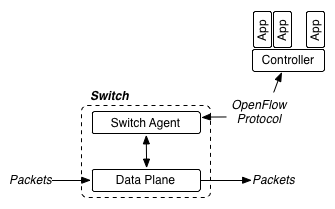
\includegraphics[width=1.0\linewidth]{of-switch-anatomy}
 	\caption{OpenFlow Switch Anatomy \cite{Of_Switch_img}} \label{fig:Of_switch_anatomy}
 	\vspace{-10pt}
\end{figure}
 
\subsubsection{OpenFlow Switch Agent \cite{Opnflow_switch}} \label{Of_switch_agent}
 The figure \ref{fig:Of_switch_agent} shows how the switch agent works, its components are explained as follows.
 
\begin{figure}
 	\centering
 	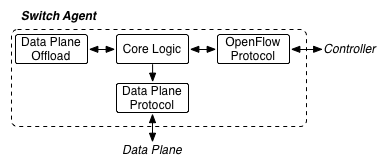
\includegraphics[width=1.0\linewidth]{of-switch-agent-anatomy}
 	\caption{OpenFlow Switch Agent \cite{Of_Switch_agent_img}} \label{fig:Of_switch_agent}
 	\vspace{-10pt}
\end{figure}

\begin{itemize}
	\item \textbf{OpenFlow protocol:} This instance is on the switch side
	\item \textbf{Core Logic:} Switch management, command execution to the data plane and manage the data plane offload etc.
	\item \textbf{Data Plane Offload:} Some functionality present in the OpenFlow will be offloaded by the control plane which is not provided in the existing data plane implementation.
	\item \textbf{Data Plane protocol:} This protocol is internal which is mostly used for configuring the data plane state.
	
\end{itemize}

\subsubsection{Data Plane \cite{Opnflow_switch}} \label{of_data_plane}

The data plane consists of the ports, flow tables, flows, classifiers and actions. Packets traverse through the system on ports. When each packet arrives, it is matched with the flows in the flow table using classifiers. The flows contain the set of actions that are applied to each packet that matches.

\begin{figure}[H]
	\centering
	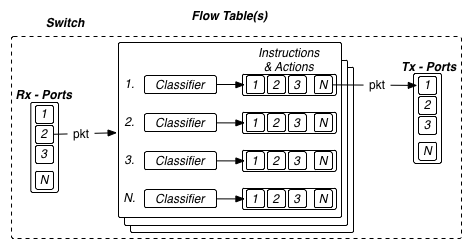
\includegraphics[width=1.0\linewidth]{Of-data-plane-flow}
	\caption{OpenFlow Data Plane Schematic \cite{Of_data_plane_flow_img}} \label{fig:Of_data_plane_img}
	\vspace{-10pt}
\end{figure}

\subsubsection{Data Plane - Packet Lifecycle \cite{Opnflow_switch}} \label{of_data_plane_lifecycle}

Each packet is processed in the following sequence as explained below.
\begin{figure}[H]
	\centering
	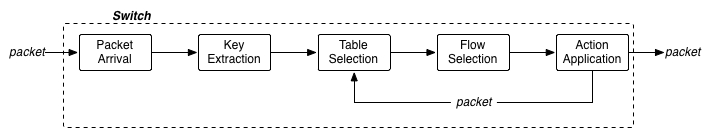
\includegraphics[width=1.0\linewidth]{Of-packet-lifecycle}
	\caption {Packet Lifecycle \cite{Of_packet_lifecycle}}
	\label{fig:of_packet_lifecycle}
	\vspace{-10pt}
\end{figure}

\begin{itemize}
	\item \textbf{Step 1: Packet Arrival}
	\\ Packets arrive in either a physical or virtual port, it is necessary to make note of the arrival port for source-based processing later.
	\item \textbf{Step 2: Key Extraction}
	\\ When each packet arrive on the port, a small meta data is built called the key. This key contains information about the packet such as header values, buffered packet, arrival port, arrival time etc. 

	\item \textbf{Step 3: Table Selection}
	\\ When a packet goes through the pipeline, the packet is matched with the first table by default and if multiple tables exist then subsequent tables will be selected through hit or miss actions.
	\item \textbf{Step 4: Flow Selection}
	\\ The Key extracted in the initial step is used for selecting the flow from the table. The first flow where the classifier subsumes the key become the selected flow.
	\item \textbf{Step 5: Application Selection}
	\\ Each flow contains a set of actions, which is applied to the packet when a flow is matched. The actions can modify the state of the packet or change how the packet is treated. 
	
\end{itemize}

\subsection{RADIUS \cite{RADIUS_RFC2865}} \label{RADIUS}
RADIUS stands for Remote Authentication Dial-In User Service, which is an access control server for authentication and accounting protocol. RADIUS is an AAA protocol used for network access applications.
\subsubsection{What is AAA Protocol? \cite{RADIUS_AAA}} \label{RADIUS_AAA}
AAA stands for Authentication, Authorization and Accounting. \textit{Authentication} is the validation of the user requesting access to a service.It is normally done by providing some credentials such as username and password. \textit{Authorization} provides specific services based on the user’s authentication such as physical location restrictions, multiple login access restrictions etc. \textit{Accounting} keeps track of all the users and their network resource consumption is provided by the accounting service, it’s like a log for every user who gained access to the network. Typical information includes user identity, nature of service delivered etc. This information may probably be used for billing, management purposes.  
%\begin{itemize}
%	\item \textbf{Authentication:} It is the confirmation to the validation of the user who is requesting a service. It is normally done by providing some credentials such as username and password.
%	\item \textbf{Authorization:} Providing specific services based on the user’s authentication such as physical location restrictions, multiple login access restrictions etc.
%	\item \textbf{Accounting:} keeping track of all the users and their network resource consumption is provided by the accounting service, it’s like a log for every user who gained access to the network. Typical information includes user identity, nature of service delivered etc. This information may probably be used for billing, management purposes.
%	
%\end{itemize}
\subsubsection{Key Features of RADIUS: \cite{RADIUS_RFC2865}} \label{RADIUS_features}

The RADIUS works like a \textit{Client / Server} model. The network server acts as the client of RADIUS, which passes the user information to designated RADIUS server. The responsibilities of the radius server include receiving connection requests, authenticating users, providing all the configuration details necessary for the client to deliver service to the user.

RADIUS also provides security by encrypting the communication between the client and the RADIUS server. So,  any users credentials sent over the network is encrypted. In addition, the client and the RADIUS server transactions are authenticated over a shared secret which is never sent over the network. The RADIUS server supports several method’s for a user to authenticate such as PPP, PAP or CHAP etc.

The RADIUS is also an extensible protocol where all transactions are of variable length Attribute-value-length 3 tuples. Supports addition of new attribute values without disturbing the existing implementation of the protocol.


%\begin{itemize}
%	\item \textbf{Client / Server Model:} 
%	\\	The network server acts as the client of RADIUS, which passes the user information to designated RADIUS server. The responsibilities of the radius server include receiving connection requests, authenticating users, providing all the configuration details necessary for the client to deliver service to the user.
%	\item \textbf{Network Security:}
%	\\ The communication between the client and the RADIUS server is encrypted so, any user password sent is encrypted. In addition, the client and the RADIUS server transactions are authenticated over a shared secret which is never sent over the network.
%	\item \textbf{Flexible Authentication Mechanisms:}
%	\\ The RADIUS server supports several method’s for a user to authenticate such as PPP, PAP or CHAP etc.
%	\item \textbf{Extensible Protocol:}
%	\\ All transactions are of variable length Attribute-value-length 3 tuples. Supports addition of new attribute values without disturbing the existing implementation of the protocol.
%	
%\end{itemize}

\subsubsection{RADIUS Components \cite{RADIUS_components}} \label{RADIUS_components}
The following components are part of the RADIUS infrastructure.
\begin{itemize}
	\item Access Clients:
	\\ These are the devices such as a mobile phone, laptop, desktop computer etc. that is requesting to gain access to the network 
	\item Access Servers (RADIUS clients):
	\\ They are network access servers such as access points, 802.1x capable switches etc. These devices communicate with the network access servers using the RADIUS protocol. They are the devices to which the clients are associated to for access to the network.
	\item RADIUS servers:
	\\ It is the network access server that manages the users and the services associated to each user or client.
	\item RADIUS proxies
	\\ They are similar to the network access server except that, they do not process the AAA information received from the RADIUS clients. They simply forward the information to the RADIUS server or to another RADIUS proxy based on the information in the packet.
	\item User account databases (Active Directory, any database such as MySQL):
	\\ It is the database to which the RADIUS server refers to (When configured to work with database) for authenticating an user requesting network access. The database also contains other accounting information such as the session details for each user, the services active for each client. 
	
\end{itemize}
The components are showing in the figure \ref{fig:RADIUS_components_img}.

\begin{figure}
	\centering
	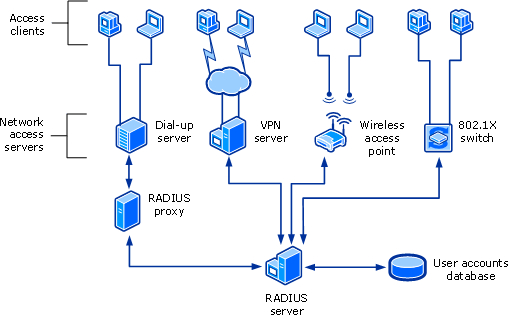
\includegraphics[width=1.0\linewidth]{RADIUS-components}
	\caption {RADIUS Components \cite{RADIUS_components_img}}
	\label{fig:RADIUS_components_img}
	\vspace{-10pt}
\end{figure}
\subsubsection{RADIUS Operation \cite{RADIUS_components}} \label{RADIUS_Operations}
RADIUS messages are sent as UDP messages using the port 1812 for authentication and port 1813 for accounting messages. Some network access servers (NAS) use 1645 and 1646 for authentication and accounting respectively.

A RADIUS data format looks as shown below where the fields are transmitted from left to right.

\begin{lstlisting}
0                   1                   2                   3
0 1 2 3 4 5 6 7 8 9 0 1 2 3 4 5 6 7 8 9 0 1 2 3 4 5 6 7 8 9 0 1
+-+-+-+-+-+-+-+-+-+-+-+-+-+-+-+-+-+-+-+-+-+-+-+-+-+-+-+-+-+-+-+-+
|     Code      |  Identifier   |            Length             |
+-+-+-+-+-+-+-+-+-+-+-+-+-+-+-+-+-+-+-+-+-+-+-+-+-+-+-+-+-+-+-+-+
|                                                               |
|                         Authenticator                         |
|                                                               |
|                                                               |
+-+-+-+-+-+-+-+-+-+-+-+-+-+-+-+-+-+-+-+-+-+-+-+-+-+-+-+-+-+-+-+-+
|  Attributes ...												|
+-+-+-+-+-+-+-+-+-+-+-+-+-+-+-+-+-+-+-+-+-+-+-+-+-+-+-+-+-+-+-+-+

\end{lstlisting}

The code field as shown in the data frame above uses one octet which help identify the type of RADIUS packet.
\begin{itemize}
	\item \textbf{Access-Request:} Sent by the RADIUS client requesting authentication and authorization for a connection.
	\item \textbf{Access-Accept:} It’s the response from the RADIUS server to the client stating that the connection was authenticated and authorized.
	\item \textbf{Access-Reject:} It’s a response from the RADIUS server to the client that the connection attempt failed in authentication.
	\item \textbf{Access-Challenge:} Sometimes the RADIUS server requires more information from the client and sends a challenge as a response the Access-Request message.
	\item \textbf{Accounting-Request:} Sent by the RADIUS client to specify accounting information for an accepted connection.
	\item \textbf{Accounting-Response:} The RADIUS server sends the acknowledgement for the successful receipt and processing of the Accounting-Request message.
	
\end{itemize}

\subsubsection{RADIUS Authentication Mechanism} \label{RADIUS_auth_mechanism}
RADIUS uses the following message codes when communicating between the RADIUS client and server as shown in the figure below.

\begin{figure}[H]
	\centering
	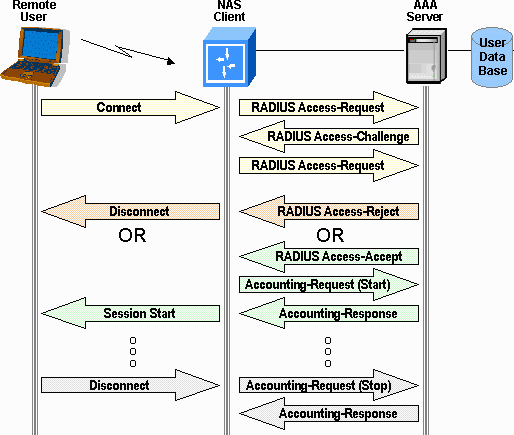
\includegraphics[width=1.0\linewidth]{radius-operation}
	\caption {RADIUS Architecture \cite{Radius_operation_img}}
	\label{fig:RADIUS_architecture}
	\vspace{-10pt}
\end{figure}

\begin{itemize}
	\item \textbf{STEP 1:}When a user makes a connection request, the NAS client sends an Access-Request message to the AAA server, in this case a RADIUS server.
	\item \textbf{STEP 2:}The RADIUS sever responds by sending an Access-Challenge message requesting more information from the user.
	\item \textbf{STEP 3:}The client responds with an Access-Request message with the requested information back to the RADIUS server. The response is typically a username and password information in the form of PPP, PAP or CHAP authentication mechanisms.
	\item \textbf{STEP 4:}The RADIUS server once after validating the received information sends back an Access-Accept information. If not validated, then it sends a Access-Reject message back to the client.
	\item \textbf{STEP 5:}Upon successfully establishing a connection, the client sends an Accounting-Request message to request to start accounting the user.
	\item \textbf{STEP 6:}The RADIUS server responds by sending an Accounting-Response message after successfully starting an accounting session for the connection. Thus, concludes the connection process of the user to the network.
	
\end{itemize}

\subsection{WLAN 802.1x Security \cite{WLAN_802.1x}} \label{802.1x}
Wi-Fi or Wireless Local Area Networks (WLAN’s) have become increasingly more popular in the recent years. The wireless standard IEEE 802.11 has become the most widely adopted standards for wireless broadband internet access. The security considerations however are more complicated in the wireless environment compared to the wired ones. IEEE 802.11 has defined the following two basic security mechanisms for secure access to wireless network.
\begin{itemize}
	\item Entity authentication including shared key and open-system.
	\item Wired Equivalent Privacy (WEP)
\end{itemize}
Both these mechanisms are proven to be severely vulnerable. To enhance the security in wireless networks, 802.11i standard was proposed. This 802.11i standard defines encryption and authentication improvements in addition to introducing protocols for key management and establishment. 802.11i also incorporates the IEEE 802.1x standard as its authentication enhancement. The IEEE 802.1x is a port based network access control used for authenticating and authorizing devices connected by various LAN’s.

The IEEE 802.1x standard is based upon the Extensible Authentication Protocol (EAP), and can use a number of authentication mechanisms which is beyond the scope of the IEEE 802.1x standard. Many authentication mechanisms such as EAP/MD5(port based) , TLS, TTLS, and PEAP can be used. The IEEE 802.1x uses EAP over LAN (EAPoL) for encapsulating EAP messages between the authenticator and the supplicant. 

There are three main components in the IEEE 802.1x system namely, the supplicant, authenticator and the authentication server. In case of WLAN, the supplicant is usually the mobile device or node, the Access Point (AP) serves as the authenticator and the RADIUS server as the authentication server.  The Port Access Entity (PAE) authenticator relays all the messages between the authentication server and the supplicant. 802.1x is used in this place to enforce the specific authentication mechanism. 

\subsubsection{802.1x Authentication Process} \label{WLAN_802.1x_auth}
Authentication methods of 802.1x include PEAP, MD5 etc. Each method has its own authentication process. The following figure shows the basic EAP based authentication process in Eduroam networks. 

\begin{figure}[H]
	\centering
	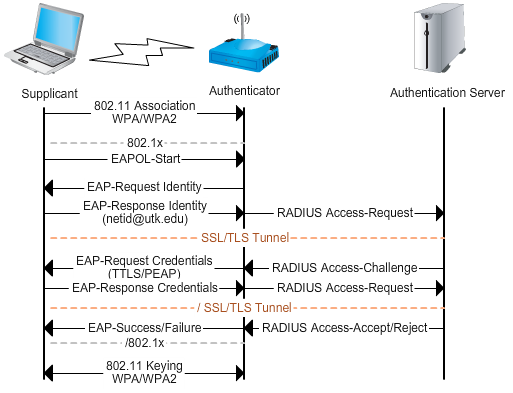
\includegraphics[width=1.0\linewidth]{WLAN_8021x_Auth}
	\caption {IEEE 802.1x WLAN authentication process \cite{WLAN_802.1x_img}}
	\label{fig:WLAN_802.1x_auth_img}
	\vspace{-10pt}
\end{figure}

\begin{itemize}
	\item \textbf{Step 1:} 
	\\ After the association of the supplicant with the authenticator or AP via WPA or WPA2 enterprise, the 802.1x application initiates the EAPOL start message with the authenticator. 
	\item \textbf{Step 2:} 
	\\ The authenticator responds by send a EAP-Request identity message from the supplicant. 
	\item \textbf{Step 3:}
	\\ Once receiving the username as a EAP response from the supplicant, the authenticator then initiates a RADIUS Access-request message with the authentication server. 
	\item \textbf{Step 4:}
	\\ The authenticator receives the RADIUS access challenge from the authentication server and forwards that via a secure SSL/TLS tunnel to the supplicant by encapsulating the EAP-Request credentials message with TTLS/PEAP.
	\item \textbf{Step 5:}
	\\ The supplicant responds with a EAP-Response Credentials message which is typically a username and password to the authenticator via the same secure tunnel, the authenticator forwards the received information as a RADIUS Access-Request message with encapsulation to the authentication server. 
	\item \textbf{Step 6:}
	\\ The authentication server responds with a RADIUS Access-Accept/Reject message to the authenticator. The Authenticator sends this information as a EAP Success/Failure message to the supplicant. 
	\item \textbf{Step 7:}
	\\ The supplicant is now fully associated with the network.
	
\end{itemize}

%	% !TEX root       = ./type_name.tex
% !TEX program    = pdflatex
% !TEX encoding   = utf-8
% !TEX spellcheck = de_DE_frami
%=======================================================================

\chapter{Standard Nova Scheduling Algorithm}\label{ch:novaalgorithm}

OpenStack Nova uses the \verb|nova-scheduler| service to determine how to dispatch the compute requests which are requested by the user.
It calculates and determines on which \verb|compute| host node should the request for the virtual machine be processed.
The scheduler can be configured through a variety of options provided by the OpenStack.


\section{Theory of Nova Algorithm}\label{sec:novaalgorithmtheory}

As explained in \nameref{sec:novafilterschedulerdetailed}, the nova scheduler has a \textbf{Filter Scheduler} which supports the filtering and weighting the hosts to make informed decisions about on which host a new instance should or can possibly be created.

The filter scheduler iterates over each host and validates if the available resources on the host can support the requested virtual instance.
It creates a list of available hosts hosts which can serve the request to host an instance and proceeds with the filter mechanism.

The filter scheduler iterates over each available host, collects the resource information from the host and weighs according to the highest to lowest resource availability.

This filter scheduler in the Compute scheduler service is configured with the following default scheduler options in the \verb|/etc/nova/nova.conf| file:

\begin{lstlisting}[frame=single]
scheduler_driver_task_period = 60
scheduler_driver = nova.scheduler.filter_scheduler.FilterScheduler
scheduler_available_filters = nova.scheduler.filters.all_filters
scheduler_default_filters = RetryFilter, AvailabilityZoneFilter, RamFilter,DiskFilter, ComputeFilter, ComputeCapabilitiesFilter, ImagePropertiesFilter, ServerGroupAntiAffinityFilter, ServerGroupAffinityFilter
\end{lstlisting}

By default, the \verb|scheduler_driver| is configured with a filter scheduler which can be found at \verb|/usr/lib/python2.7/dist-packages/nova/scheduler/filter_sche|- \verb|duler.py| with the class name \verb|FilterScheduler|.

In the default configuration, this scheduler considers hosts that meet all the following criteria:

\begin{itemize}
	\item Any host that has not been attempted for scheduling purposes (RetryFilter).

	\item Any host that is available in the requested availability zone (AvailabilityZoneFilter).

	\item Any host that has sufficient availability of RAM to host an instance (RamFilter).

	\item Any host that has sufficient disk memory space available for root and ephemeral storage (DiskFilter).

	\item Any host that can and is available to service the request (ComputeFilter).

	\item Any host that can satisfy the extra specifications associated with the instance type (ComputeCapabilitiesFilter).

	\item Any host that can satisfy any architecture, hypervisor type, or virtual machine mode properties specified on the instance's image properties (ImagePropertiesFilter).

	\item Any host that is on a different host than other instances of a group (if requested) (ServerGroupAntiAffinityFilter).

	\item Any host that is in a set of group hosts (if requested) (ServerGroupAffinityFilter).

	\item Any host that is visible in the refreshed scheduler cache list of available hosts; by the use of \verb|scheduler_driver_task_period| option to specify how often the list is updated.
\end{itemize}

When the task of scheduling a virtual machine on a host is triggered by an user, the Filter Scheduler iterates over all found compute nodes, evaluating each against a set of filters.
The resultant list of available hosts are ordered by the weighers.

At the end, the Filter Scheduler sorts selected hosts by their weight and attempts to provision instances on the chosen hosts.

\newpage

\section{Code Trace}\label{sec:codetrace}

In this section, the code trace to the nova scheduler can be observed.

When an instance is requested, it is received by the nova API listener for validation of the nova API URL and processes the requested tasks based on the requested input parameters.
The Nova API reads the default scheduler file from the \verb|/etc/|\verb|nova/| \verb|nova.conf| file.
In the python source file \verb|filter_scheduler|, the \verb|FilterScheduler| \verb|class| is initialized by the \verb|driver.Scheduler| driver.

The scheduler driver object calls the \verb|def| \verb|select_destinations(self,| \verb|context,| \verb|request_spec,| \verb|filter_properties)| function in the \verb|FilterScheduler| class.
\newline
\begin{lstlisting}[frame=single, language=Python, caption={The function select\_destination},label={lst:select_destinations}, escapechar=|]
def select_destinations(self, context, request_spec, filter_properties):
	"""Selects a filtered set of hosts and nodes."""
	self.notifier.info(context,
		'scheduler.select_destinations.start',
		dict(request_spec=request_spec))

	# Count of requested virtual instances
	num_instances = request_spec['num_instances']

	# The FilterScheduler._schedule function is called,
	# which schedules the possible hosts for the requested instances
	selected_hosts = self._schedule(context, request_spec,|\label{line:select_destinations_schedule}|
		filter_properties)

	...
	...
	
\end{lstlisting}

In the above code listing \ref{lst:select_destinations}, the function \verb|_schedule| called at line \ref{line:select_destinations_schedule}
initiates the scheduling algorithm by passing the \verb|request_spec| as the parameter which holds all the specifications for creating the virtual instances like; requested number of instances, required RAM capacity per instance, required HDD capacity per instance, required VCPUs per instance, required OS image to boot the virtual instance with it, and other instance related parameters.

Stepping into the function \verb|FilterScheduler._schedule| given in listing \ref{lst:select_destinations_schedule}.
\newline
\begin{lstlisting}[frame=single, language=Python, caption={The function \_schedule}, label={lst:select_destinations_schedule}, escapechar=|]
def _schedule(self, context, request_spec, filter_properties):
	"""Returns a list of hosts that meet the required specs,
	ordered by their fitness.
	"""

	...
	...
	
	# iterate each host and select the host to place an instance
	for num in range(num_instances):
		# Filter local hosts based on requirements ...
		hosts = self.host_manager.get_filtered_hosts(hosts,|\label{line:get_filtered_hosts}|
				filter_properties, index=num)
		if not hosts:
			# Can't get any more locally.
			break

		LOG.debug("Filtered %(hosts)s", {'hosts': hosts})

		# weigh the hosts based on the weighing filter
		weighed_hosts = self.host_manager.get_weighed_hosts(hosts,|\label{line:get_weighed_hosts}|
				filter_properties)

		...
		...
		
		chosen_host = random.choice(
			weighed_hosts[0:scheduler_host_subset_size])
		LOG.debug("Selected host: %(host)s", {'host': chosen_host})
		selected_hosts.append(chosen_host)|\label{line:chosen_host}|

		...
		...

	LOG.info('%s number of instances scheduled with filter scheduler in %s seconds' % (num_instances, (rtime.time() - start_time)))
	return selected_hosts
\end{lstlisting}


In the listing \ref{lst:select_destinations_schedule}, at the line number \ref{line:get_filtered_hosts}, the function \verb|get_filtered_hosts| in the class \verb|HostManager| in the python source file \verb|host_manager| is called to filter the hosts based on the RAM filter, Disk Filter, Compute Filter, and other specified filters in the list.

Stepping into the \verb|get_filtered_hosts| given in listing \ref{lst:get_filtered_hosts}.
\newline
\begin{lstlisting}[frame=single, language=Python, caption={The function get\_filtered\_hosts}, label={lst:get_filtered_hosts}, escapechar=|]
def get_filtered_hosts(self, hosts, filter_properties,
		filter_class_names=None, index=0):
	"""Filter hosts and return only ones passing all filters."""

	...
	...
	
	if filter_class_names is None:
		filters = self.default_filters|\label{line:default_filters}|
	else:
		filters = self._choose_host_filters(filter_class_names)|\label{line:choose_host_filters}|
	ignore_hosts = filter_properties.get('ignore_hosts', [])
	force_hosts = filter_properties.get('force_hosts', [])
	force_nodes = filter_properties.get('force_nodes', [])

	...
	...
	return self.filter_handler.get_filtered_objects(filters,
			hosts, filter_properties, index)
\end{lstlisting}

In this listing \ref{lst:get_filtered_hosts}, the filter classes are loaded either by default at line number \ref{line:default_filters} or by the specified list of filters at line number \ref{line:choose_host_filters}.
These classes include the \verb|nova|.\verb|scheduler|. \verb|filters|.\verb|ram_filter|, \verb|nova|.\verb|scheduler|.\verb|filters|.\verb|disk_filter|, \verb|nova|.\verb|scheduler|.\newline\verb|filters|.\verb|compute_filter| and other specified default filters.

In the listing \ref{lst:select_destinations_schedule}, at the line number \ref{line:get_weighed_hosts}, the function \verb|get_weighed_hosts| in the class \verb|HostManager| in the python source file \verb|host_manager| is called to get list of hosts sorted according to the weights calculated by the weights filter. At line \ref{line:chosen_host} the chosen host is then set as selected host for the requested virtual instance.

The listing \ref{lst:get_weighed_hosts} calculates the weights of each host by comparing with the available properties of host and the requested properties of an instance as mentioned in the section \ref{ssec:novaweights}
\begin{lstlisting}[frame=single, language=Python, caption={The function \_schedule}, label={lst:get_weighed_hosts}, escapechar=|]
def get_weighed_hosts(self, hosts, weight_properties):
	"""Weigh the hosts."""
	return self.weight_handler.get_weighed_objects(self.weighers,
			hosts, weight_properties)
\end{lstlisting}

The \verb|get_weighed_objects| looks for actual available resources on the hosts and calculates the weight of each objects.

The custom trace of the log can be observed in the Appendix \nameref{app:ch:logs} at \nameref{app:sec:filterschedulerlogtrace}.
	% !TEX root       = ./type_name.tex
% !TEX program    = pdflatex
% !TEX encoding   = utf-8
% !TEX spellcheck = de_DE_frami
%=======================================================================

\chapter{Implementation of Cplex based Nova Scheduler}\label{ch:implementationofcplex}

After the iterations of debugging the OpenStack Scheduler Python module, the key parameters which contribute in the calculation of the placement decisions of virtual instances are identified.
The key parameters that would be required in computation of placements decision are:
\begin{itemize}
	\item Available RAM capacity on each of the Compute node and
	\item Available Hard Disk capacity on each of the Compute node
\end{itemize}

The number of CPU cores are not taken into consideration.
As the Compute nodes support the hardware acceleration for virtual machines using the KVM mode, the CPU cores can be over utilised.
The default \verb|cpu_allocation_ratio| is set to 16 which allows the over creation of virtual CPU cores, due to which the available CPU cores do not play a major role in determining the creation of virtual instances.

In this chapter, the formulation of the new cPlex based Mathematical model is explained,
and also the implemented code is provided with an explanation.

\section{Mathematical Formulation}\label{sec:mathematicalformulation}
The idea behind the mathematical formulation is to implement the energy efficient scheduler mechanism, where the placement decisions are made to utilise maximum capacity of the Compute node before a new placement decision is requested on the other Compute nodes. This was conceptualised with an idea to extend the algorithm with an ability to perform live migration of the existing virtual machines to re-order the placement decisions.

As the live migration is still a work in progress, the mathematical model is formulated with only the essential parameters into considerations.

Parameters for the mathematical model are defined as follows:
\\$n_s$ is the host number in the set of nodes.
\\$N_s$ is the set of all the host nodes.
\\$n_v$ is the virtual instance number in the requested virtual instances list.
\\$N_v$ is the set of all the requested virtual instances to be placed.
\\$x_{n_s}$ is the each individual host node.
\\$x_{n_s}^{n_v}$ is the unique combination of requested virtual instance from the set of $N_v$ and host node from the set of $N_s$.
\\$suit_{n_s}^{n_v}$ is the suitable host entry for the requested virtual instance.
\\$d_{n_v}^{RAM}$ is the required demand of RAM for the given virtual instance.
\\$c_{n_s}^{RAM}$ is the available capacity of RAM in the given host node.
\\$d_{n_v}^{HDD}$ is the required demand of hard disk for the given virtual instance.
\\$c_{n_s}^{HDD}$ is the available capacity of hard disk in the given host node.

The objective function is to minimize the host nodes for placing the requested virtual instances. 
This objective function can be given as:
\begin{equation} \label{eq:1}
\min{\sum_{n_s \in N_s}{x_{n_s}}}
\end{equation}

For each virtual instance, the placement request of the virtual instance is done on one and only one host node. This can be given by the equation:
\begin{equation} \label{eq:2}
\sum_{n_s \in N_s}{x_{n_s}^{n_v}}{suit_{n_s}^{n_v}} = 1, \forall{n_v} \in N_v
\end{equation}

The equation to determine if the host is suitable or not suitable for a given combination of virtual instance and host is given by:
\begin{equation} \label{eq:3}
x_{n_s}^{n_v} \leq suit_{n_s}^{n_v},\forall{n_s} \in N_s, n_v \in N_v
\end{equation}

The equation which evaluates if the placement decision can be made on the given host node or not for a given virtual instance is given by:
\begin{equation} \label{eq:4}
x_{n_s} \geq x_{n_s}^{n_v},\forall{n_s} \in N_s, n_v \in N_v
\end{equation}

The RAM capacity constraints are given as follows:
\begin{equation} \label{eq:5}
\sum_{n_v \in N_v}{x_{n s}^{n_v}}{d_{n_v}^{RAM}} \leq c_{n_s}^{RAM}, \forall{n_s} \in N_s 
\end{equation}

The hard disk(HDD) capacity constraints are given as follows:
\begin{equation} \label{eq:6}
\sum_{n_v \in N_v}{x_{n s}^{n_v}}{d_{n_v}^{HDD}} \leq c_{n_s}^{HDD}, \forall{n_s} \in N_s 
\end{equation}

These equations provide the boundary conditions to determine the possible placement decision of the virtual instances in the host nodes.

\section{The overview of implementation}\label{sec:overviewofimplementation}

IBM ILOG CPLEX\textsuperscript{\textregistered} Optimizer is a mathematical programming technology that enables decision of mathematical optimization for improving efficiency, reducing costs, and increasing profitability\cite{cplex-optimizer}.
This software is used to provide the solution for placement decision of the virtual instances on the host nodes.
For the purpose of this Thesis, the version 12.6 of the IBM Cplex is used.

To implement the mathematical formulation described in the section \nameref{sec:mathematicalformulation}, a new scheduler file is created with a name \verb|"tuc_ccn_scheduler.py"|.

The \verb|tuc_ccn_scheduler.py| has the class and function definition similar to the default \verb|FilterScheduler|.
There are few changes in the implementation of the \verb|_schedule| function and a new function named as \verb|solve_TUC_Cplex| has been added to implement the new cPlex based mathematical scheduling model.

The \verb|_schedule| function for the new \verb|tuc_ccn_scheduler| is given as:
\newline
\begin{lstlisting}[frame=single, language=Python, caption={The cPlex based TUC\_scheduler's \_schedule function}, label={lst:tuc_schedule}, escapechar=|]
def _schedule(self, context, request_spec, filter_properties):
	"""Returns a list of hosts that meet the required specs,
	ordered by their fitness.
	"""
	elevated = context.elevated()
	instance_properties = request_spec['instance_properties']

	# NOTE(danms): Instance here is still a dict, which is converted from
	# an object. The pci_requests are a dict as well. Convert this when
	# we get an object all the way to this path.
	# TODO(sbauza): Will be fixed later by the RequestSpec object
	pci_requests = instance_properties.get('pci_requests')
	if pci_requests:
		pci_requests = (
			objects.InstancePCIRequests.from_request_spec_instance_props(
				pci_requests))
		instance_properties['pci_requests'] = pci_requests

	instance_type = request_spec.get("instance_type", None)

	update_group_hosts = filter_properties.get('group_updated', False)

	config_options = self._get_configuration_options()

	filter_properties.update({'context': context,
							  'request_spec': request_spec,
							  'config_options': config_options,
							  'instance_type': instance_type})

	# Find our local list of acceptable hosts by repeatedly
	# filtering and weighing our options. Each time we choose a
	# host, we virtually consume resources on it so subsequent
	# selections can adjust accordingly.

	# Note: remember, we are using an iterator here. So only
	# traverse this list once. This can bite you if the hosts
	# are being scanned in a filter or weighing function.
	hosts = self._get_all_host_states(elevated)
	selected_hosts = []
	num_instances = request_spec.get('num_instances', 1)

	# the function get_filtered_hosts is called only once
	# before the for loop unlike the default scheduler's
	# _schedule function
	hosts = self.host_manager.get_filtered_hosts(hosts,|\label{line:tuc_get_filtered_hosts}|
			filter_properties, index=0)

	weighed_hosts = self.weight_handler.get_weighed_objects(self.weighers,
			hosts, filter_properties)

	vi_hosts = {}
	start_time = rtime.time()
	# implementation of cPlex based mathematical solver
	try:
		vi_hosts = self.solve_TUC_Cplex(hosts, filter_properties, num_instances)|\label{line:solve_TUC_Cplex}|
	except CplexError as exc:
		LOG.error('%s', exc)
		reason = _(exc)
		raise exception.NoValidHost(reason=reason)
	#end of the function call within try and exception
	
	for num in range(num_instances):
		weighed_hosts = vi_hosts[num]

		scheduler_host_subset_size = CONF.scheduler_host_subset_size

		if scheduler_host_subset_size > len(weighed_hosts):
			scheduler_host_subset_size = len(weighed_hosts)
		if scheduler_host_subset_size < 1:
			scheduler_host_subset_size = 1

		chosen_host = weighed_hosts[0]
		LOG.debug("Selected host: %(host)s", {'host': chosen_host})

		# append the selected hosts  to the array mapping
		selected_hosts.append(chosen_host)

		# Now consume the resources so the filter/weights
		# will change for the next instance.
		chosen_host.obj.consume_from_instance(instance_properties)
		if update_group_hosts is True:
			# NOTE(sbauza): Group details are serialized into a list now
			# that they are populated by the conductor, we need to
			# deserialize them
			if isinstance(filter_properties['group_hosts'], list):
				filter_properties['group_hosts'] = set(
					filter_properties['group_hosts'])
			filter_properties['group_hosts'].add(chosen_host.obj.host)
	LOG.info('%s number of instances scheduled with tuc scheduler in %s seconds' % (num_instances, (rtime.time() - start_time)))
	return selected_hosts
\end{lstlisting}

In the above code listing \ref{lst:tuc_schedule}, the \verb|get_filtered_hosts| at line number \ref{line:tuc_get_filtered_hosts} is called before the for loop and called only once to provide an input to cPlex solver, unlike the default scheduler which filters the hosts for each request of an instance.

The cPlex based solver funtion is called at line number \ref{line:solve_TUC_Cplex}. The hosts, filter\_properties and num\_instances are passed as parameters to the function in the listing \ref{lst:solve_TUC_Cplex}.
\newline
\begin{lstlisting}[frame=single, language=Python, caption={The cPlex based TUC\_scheduler's solve\_TUC\_Cplex function}, label={lst:solve_TUC_Cplex}, escapechar=|]
def solve_TUC_Cplex(self, hosts, filter_properties, num_instances):
	weighedHosts    = []
	#available RAM capacity on each compute (host) node
	ns_rams         = []
	#available HDD capacity on each compute (host) node
	ns_hdds         = []
	for host in hosts:
		weighedHost = []
		weighedHost.append(host)
		weighedHost = self.host_manager.get_weighed_hosts(weighedHost,
				filter_properties)
		weighedHosts.append(weighedHost)
		ns_rams.append(host.free_ram_mb)
		ns_hdds.append(host.free_disk_mb)

	instance_type = filter_properties['instance_type']
	root_gb     = instance_type['root_gb']
	memory_mb   = instance_type['memory_mb']
	nvram       = 1.0*memory_mb
	nvhdd       = 1024.0*root_gb
	my_prob     = cplex.Cplex()

	#Number of hosts available to cater the requested instances
	host_count  = len(hosts)
	vis         = num_instances

	# cPlex input parameters
	# objective function parameters
	my_obj      = []
	# upper bound values
	my_ub       = []
	# lower bound values
	my_lb       = []
	# parameter type
	my_ctype    = ''
	# names of all the mathematical parameters
	my_colnames = []
	# the values on the right hand side
	my_rhs      = []
	# unique name for each row
	my_rownames = []
	my_sense    = ''

	rows        =   []

	# translate the mathematical formulations into cPlex input
	for i in range(host_count):
		my_obj.append(1.0)
		my_colnames.append("x_"+str(i))
		my_ub.append(1.0)
		my_lb.append(0.0)
		my_ctype = my_ctype+'B'
		vvar  = []
		vvalr = []
		vvalh = []
		for j in range(vis):
			my_obj.append(0.0)
			my_colnames.append("x_"+str(i)+"_"+str(j))
			my_ub.append(1.0)
			my_rhs.append(0.0)
			my_ctype = my_ctype+'B'
			my_lb.append(0.0)
			row = []
			var = []
			val = []
			var.append("x_"+str(i))
			var.append("x_"+str(i)+"_"+str(j))
			val.append(1.0)
			val.append(-1.0)
			row.append(var)
			row.append(val)
			rows.append(row)
			my_rownames.append('rsv_'+str(i)+'_'+str(j))
			my_sense = my_sense+'G'
			vvar.append("x_"+str(i)+"_"+str(j))
			vvalr.append(nvram)
			vvalh.append(nvhdd)
		row = []
		row.append(vvar)
		row.append(vvalr)
		rows.append(row)
		my_rhs.append(ns_rams[i])
		my_sense = my_sense+'L'
		my_rownames.append('rsram_'+str(i))
		row = []
		row.append(vvar)
		row.append(vvalh)
		rows.append(row)
		my_rhs.append(ns_hdds[i])
		my_sense = my_sense+'L'
		my_rownames.append('rshdd_'+str(i))

	for i in range(vis):
		row = []
		var = []
		val = []
		for j in range(host_count):
			var.append("x_"+str(j)+"_"+str(i))
			val.append(1.0)
		my_sense = my_sense+'E'
		row.append(var)
		row.append(val)
		rows.append(row)
		my_rhs.append(1.0)
		my_rownames.append('rnv_'+str(i))

	my_prob.objective.set_sense(my_prob.objective.sense.minimize)

	my_prob.variables.add(obj=my_obj, lb=my_lb, ub=my_ub,
		types=my_ctype, names=my_colnames)

	# pass all parameters to cPlex to solve the equation
	my_prob.linear_constraints.add(lin_expr=rows, senses=my_sense,
		rhs=my_rhs, names=my_rownames)
	# solve the mathematical model
	my_prob.solve()

	numcols = my_prob.variables.get_num()
	numrows = my_prob.linear_constraints.get_num()

	slack = my_prob.solution.get_linear_slacks()
	# get the solution values
	x = my_prob.solution.get_values()

	vi_hosts = {}
	for i in range(vis):
		for j in range(host_count):
			vi_host = (j*vis+1+j)+i
			if x[vi_host] == 1.0:
				vi_hosts[i] = weighedHosts[j]

	#LOG.info('VI Hosts: %(vih)s', {'vih': vi_hosts})
	return vi_hosts
\end{lstlisting}

The above code listing \ref{lst:solve_TUC_Cplex} is a cPlex based approach to perform scheduling of virtual instances.

The comparisions of both the schedulers and their performances are provided in the chapter \nameref{ch:comparisionofbothscheduler}.

	% !TEX root       = ./type_name.tex
% !TEX program    = pdflatex
% !TEX encoding   = utf-8
% !TEX spellcheck = de_DE_frami
%=======================================================================

\chapter{Comparision of performance evaluation}\label{ch:comparisionofbothscheduler}

In this chapter, observations are made based on both the schedulers.
The data based on default nova scheduler driver and the data based on tuc\_scheduler driver are evaluated for different iterations of scheduling of virtual instances.
A data set of different number of virtual instance creation is performed on both of the scheduler drivers.



\section{Observations of standard Nova scheduler}\label{sec:observationsofstandardnova}

Observing the listing \ref{lst:select_destinations_schedule}, at the line \ref{line:get_filtered_hosts} it can be seen that the \verb|get_filtered_hosts| is performed for each virtual instance scheduling rather than once for the whole of the request. This is also followed by line \ref{line:get_weighed_hosts} to get weighed hosts for each virtual instance scheduling instead of once for the whole of the request.

In the log trace listing \ref{lst:filterschedulercodetracelog10vi} at the line number \ref{line:result_filter_scheduler_placement}, it can be observed that, the placement decision of the 10 virtual instances is spread across all the host systems.
This creates the need to keep the hosts powered up for all the time.

The log trace listing \ref{lst:filterschedulercodetracelog10vi} provided in the Appendix \nameref{app:ch:logs} in chapter \nameref{app:sec:filterschedulerlogtrace10vi} shows the number of times the \verb|get_filtered-| \verb|_hosts| and \verb|get_weighed_hosts| is called to calculate the placement decision of 10 virtual instances.

\begin{figure}[H]
	\begin{center}
		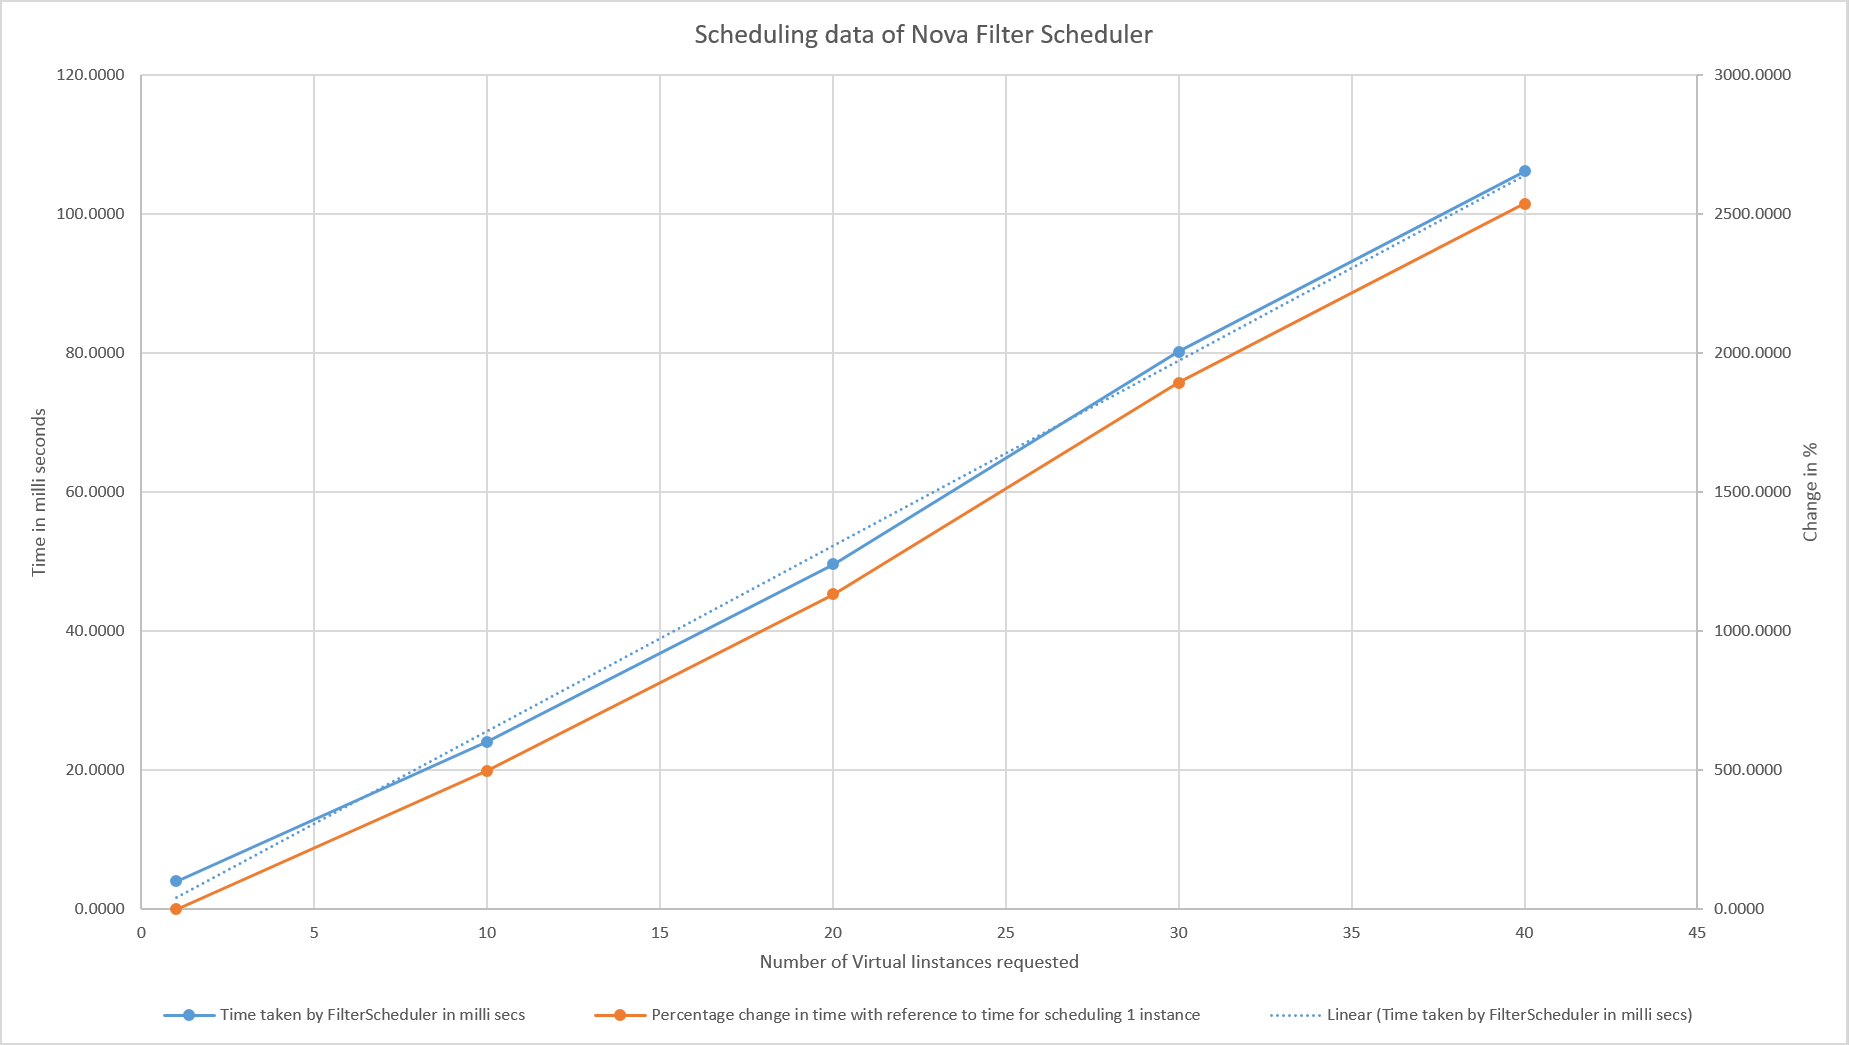
\includegraphics[width=1\linewidth]{NovaFilterSchedulerChart}
		\caption{Placement decision time for Standard Nova Scheduler from the data \ref{tabular:filterschedulerlogdata}}
		\label{fig:NovaFilterSchedulerChart}
	\end{center}
	\vspace{-10pt}
\end{figure}

The above table \ref{tabular:filterschedulerlogdata} is the time logs recorded for different requested number of virtual instances.
Here in the table, for providing a placement decision of 10 virtual instances, the standard nova scheduler takes around 24.10ms.
The percentage change in time is given by the change in time with reference to time for scheduling 1 instance.

\section{Observations of cPlex based scheduler}\label{sec:observationsoftucscheduler}

Observing the listing \ref{lst:tuc_schedule}, at the line \ref{line:tuc_get_filtered_hosts} it can be seen that the \verb|get_filtered_hosts| is executed only once for all the bulk requests of virtual instance scheduling.
This is followed by line \ref{line:solve_TUC_Cplex} \verb|solve_TUC_Cplex| to solve the scheduling problem for all the bulk requests.

In the log trace listing \ref{lst:tucschedulercodetracelog10vi} at the line number \ref{line:result_cplex_scheduler_placement}, it can be observed that, the placement decision of all the 10 virtual instances is concentrated on one host system \verb|"compute03"|.

The log trace listing \ref{lst:tucschedulercodetracelog10vi} provided in the Appendix \nameref{app:ch:logs} in chapter \nameref{app:sec:cplexschedulerlogtrace10vi} shows that only one instance of the \verb|get_filtered_hosts| is called to calculate the placement decision of 10 virtual instances.

\begin{figure}[H]
	\begin{center}
		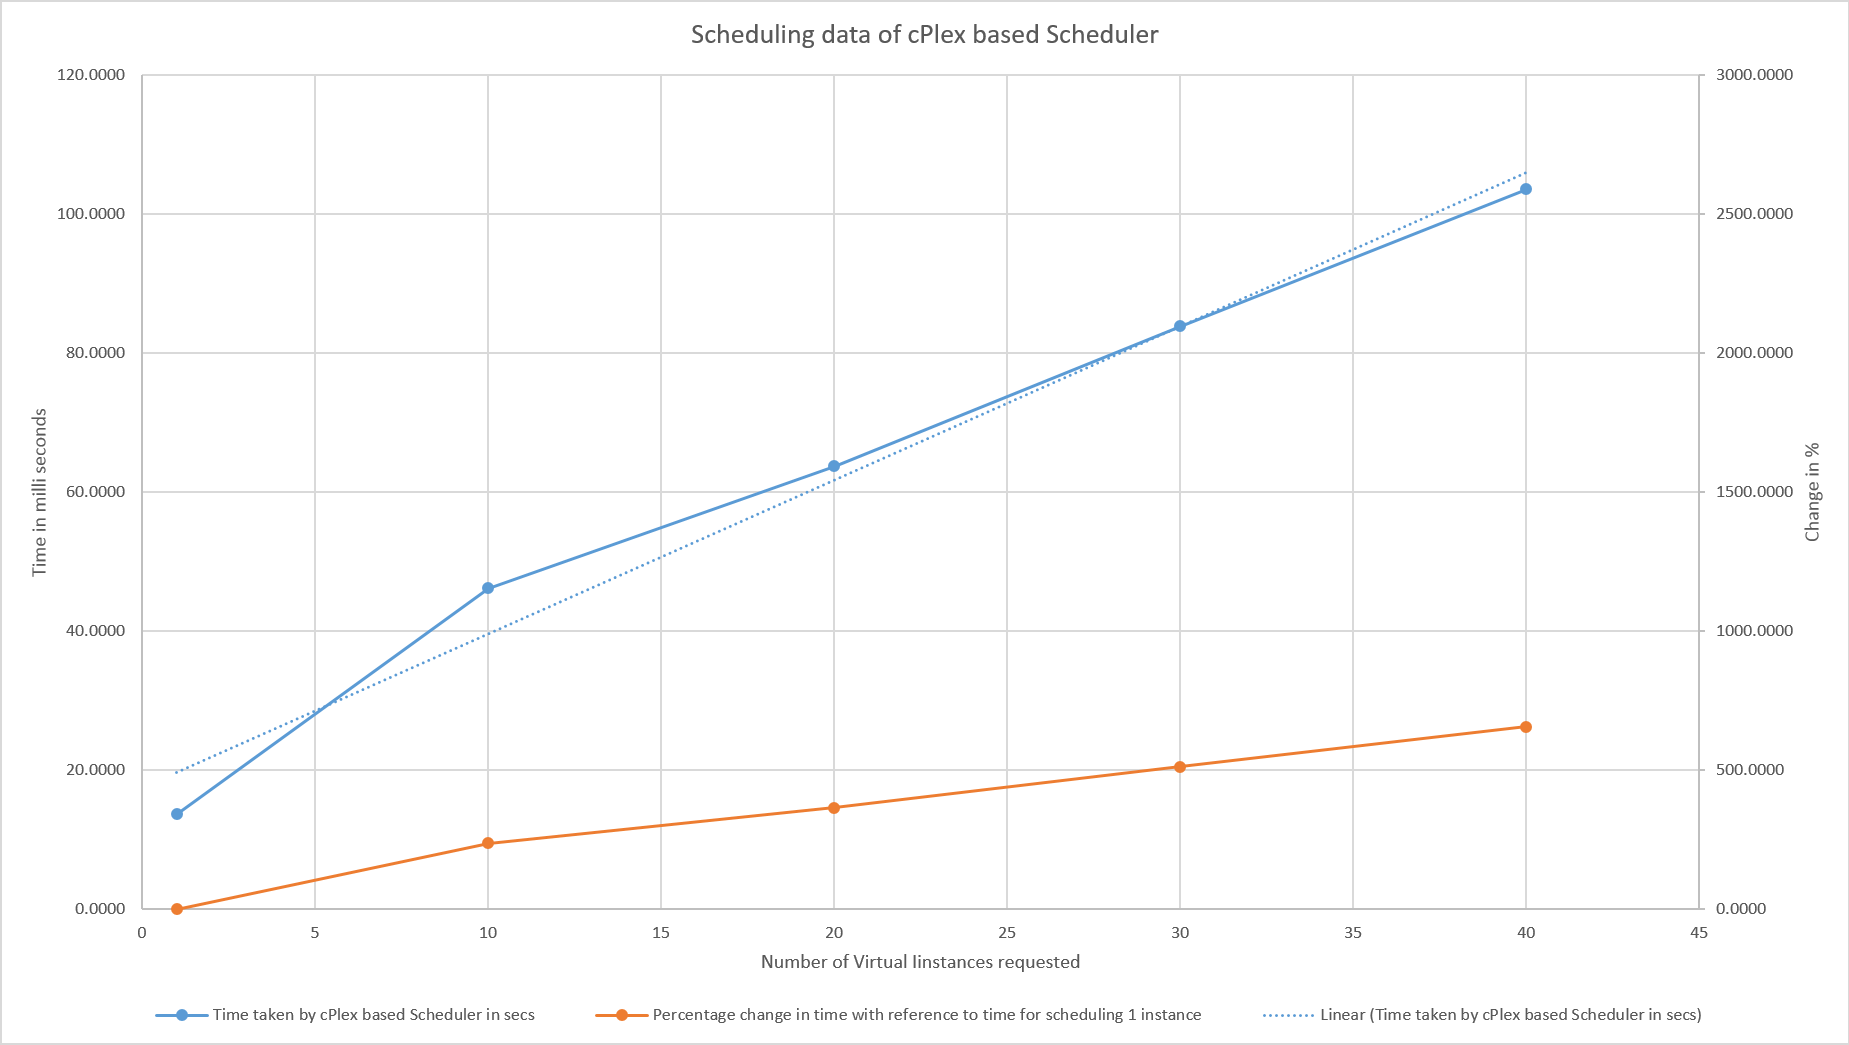
\includegraphics[width=1\linewidth]{cPlexSchedulerChart}
		\caption{Placement decision time for cPlex based Scheduler from the data \ref{tab:tucschedulerlogdata}}
		\label{fig:cPlexSchedulerChart}
	\end{center}
	\vspace{-10pt}
\end{figure}

\comment{
If the total requested capacity of RAM or HDD of virtual instances are more than the total available capacities, then the cPlex throws an exception as "unsolvable problem error". This exception is caught by the code and displayed as an error message on the screen.
}
\section{Comparision}\label{sec:comparision}

As stated in sections \nameref{sec:observationsofstandardnova} and \nameref{sec:observationsoftucscheduler}, the default Filter scheduler places the virtual instances across the hosts, whereas the \verb|tuc_ccn_scheduler| aggregates the creation of virtual instances on minimum possible host systems.
As the virtual instances on the new \verb|tuc_ccn_scheduler| are not spread across the multiple machines and aggregated on the few machines, the rest of the machines can be powered down which reduces the operating power costs.

On the other hand, combining the above two charts \ref{fig:NovaFilterSchedulerChart} and \ref{fig:cPlexSchedulerChart}, it can be observed that the slope of the cplex based scheduler is lesser than the slope of the standard nova filter scheduler. Which means that, for a larger requests of virtual instances, the cPlex based scheduler would be more efficient in providing the placement decisions for all the requested virtual instances. The initial offset time for execution of cPlex to solve the mathematical problem is higher compared to the standard nova filter scheduler.

\begin{figure}[H]
	\begin{center}
		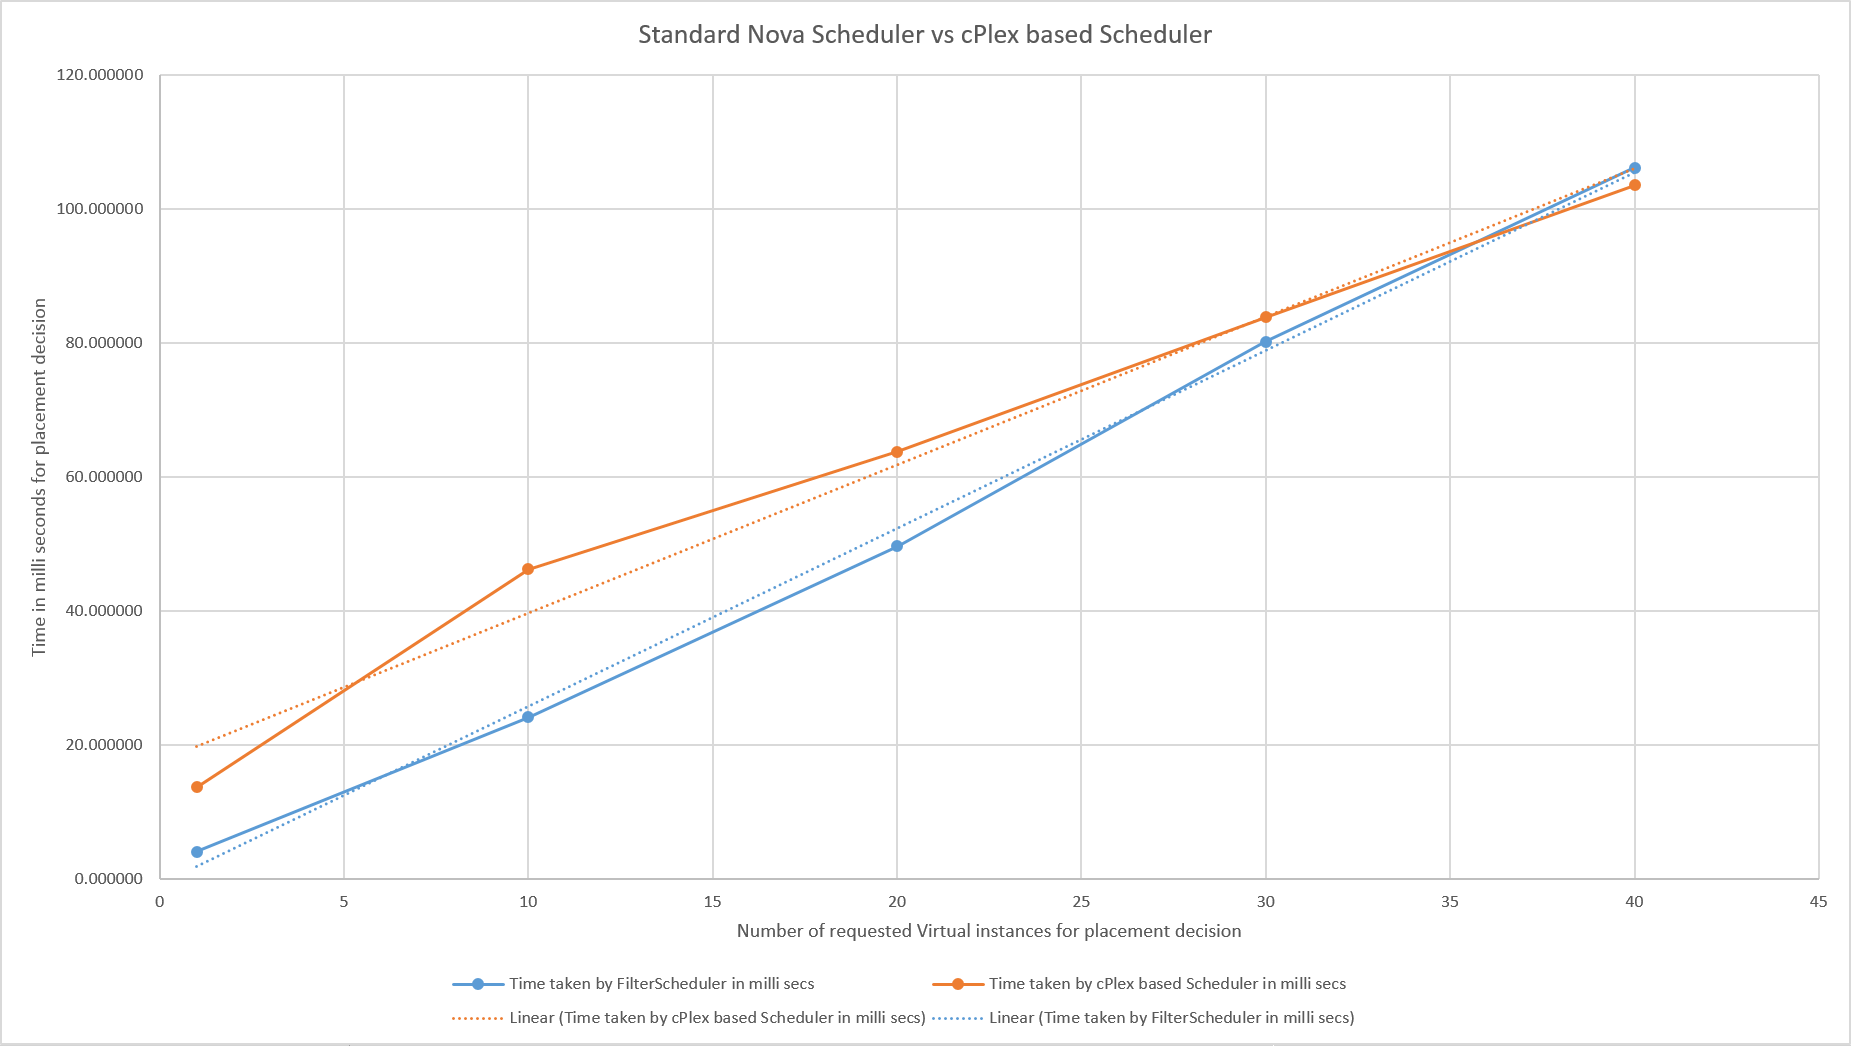
\includegraphics[width=1\linewidth]{novavscplex}
		\caption{Comparision of placement decision time between Standard Nova FilterScheduler and cPlex based Scheduler}
		\label{fig:novavscplex}
	\end{center}
	\vspace{-10pt}
\end{figure}

From the above chart \ref{fig:novavscplex}, it can be concluded that, the higher the number of requests to schedule the virtual instances the lesser the solving time for scheduling compared to the nova filter scheduler.

\section{Space for further improvements}\label{sec:spaceforimprovements}

As an example, let there be three host machines with a RAM capacity of 16GB each.
Let there be 9 virtual machines which consume 4GB of RAM each and shared equally among three host machines.
The available capacity of RAM is limited to 4GB on each machine whereas the total available capacity of RAM across all the machines is 12GB.
When there is a request for a virtual machine which requires the RAM of 8GB, both the schedulers would fail to make a placement decision for the requested virtual instance as there is no host with an available capacity of 8GB.

"Live Migration" is a functionality which would move the running virtual machine from one physical host machine to another physical host machine with minimum or no downtime.
Currently, the OpenStack Liberty has an ongoing issue with "Live Migration".
The live migration functionality fails to migrate the virtual instance from the source host machine to requested destination host machine and turns off the virtual instance scheduled for migration.
This "Live Migration" functionlity could mitigate the above mentioned issue with runtime reallocation of live(running) virtual machines to free the space by migrating it to any other possible hosts, freeing the space on the host and make a placement decision to allocate a new request of 8GB.

An idea for future could also be to have a shared resource pooling with a high speed dedicated networking bus on the hardware, to make the large clusters of compute servers into a single shared entity.
	% !TEX root       = ./type_name.tex
% !TEX program    = pdflatex
% !TEX encoding   = utf-8
% !TEX spellcheck = de_DE_frami
%=======================================================================

\chapter{Further possible extensions in OpenStack}\label{ch:futurepossibilities}
Being one of the key open source software platform for Cloud Computing in Infrastructure-as-a-Service model, it has various possible implementations and extensions.
As far as networking is concerned, there are modules in and out of OpenStack which provides the Network Functions Virtualization (NFV) for global telecom providers.

Network Functions Virtualization (NFV) allows telecom and enterprise network operators to control their networking functions: physical, virtual and functional domains—using commercial off-the-shelf hardware, and open source software as a single control pane for management and orchestration.
Here, OpenStack can provide a platform for the development and evolution of NFV components across the virtual systems. With robust system level integration and deployment a reference NFV platform can be created to accelerate the transformation of enterprise and service provider networks.

Early on, the telecommunications industries and the networking vendors have recognised the potential for OpenStack as a platform for NFV, which triggered investigations and work in development of OpenStack compatible modules to optimize for NFV.

"Network Functions Virtualization (NFV) is now synonymous with OpenStack. When people say NFV, there is an implication that they are talking about OpenStack."\cite{openstack_nfv}

Both the European Telecommunications Standards Institute and Linux Foundation collaboration project OPNFV have defined specifications and released reference platforms for NFV that select OpenStack as the Virtualization Infrastructure Manager. Additionally, OpenStack is the dominant choice for additional management and orchestration functions.\cite{nfv_technical_overview}

The interoperability between OpenStack and virtualized network functions is still an ongoing development.

So, what does Network Functions Virtualization (NFV) define?
To answer in a simple way, it is a new way to define, create, and manage networks by replacing dedicated network appliances with software and automation.
It is the idea of replacing the physical network devices which are dedicated and expensive by the virtual software devices.

\begin{figure}[H]
	\begin{center}
		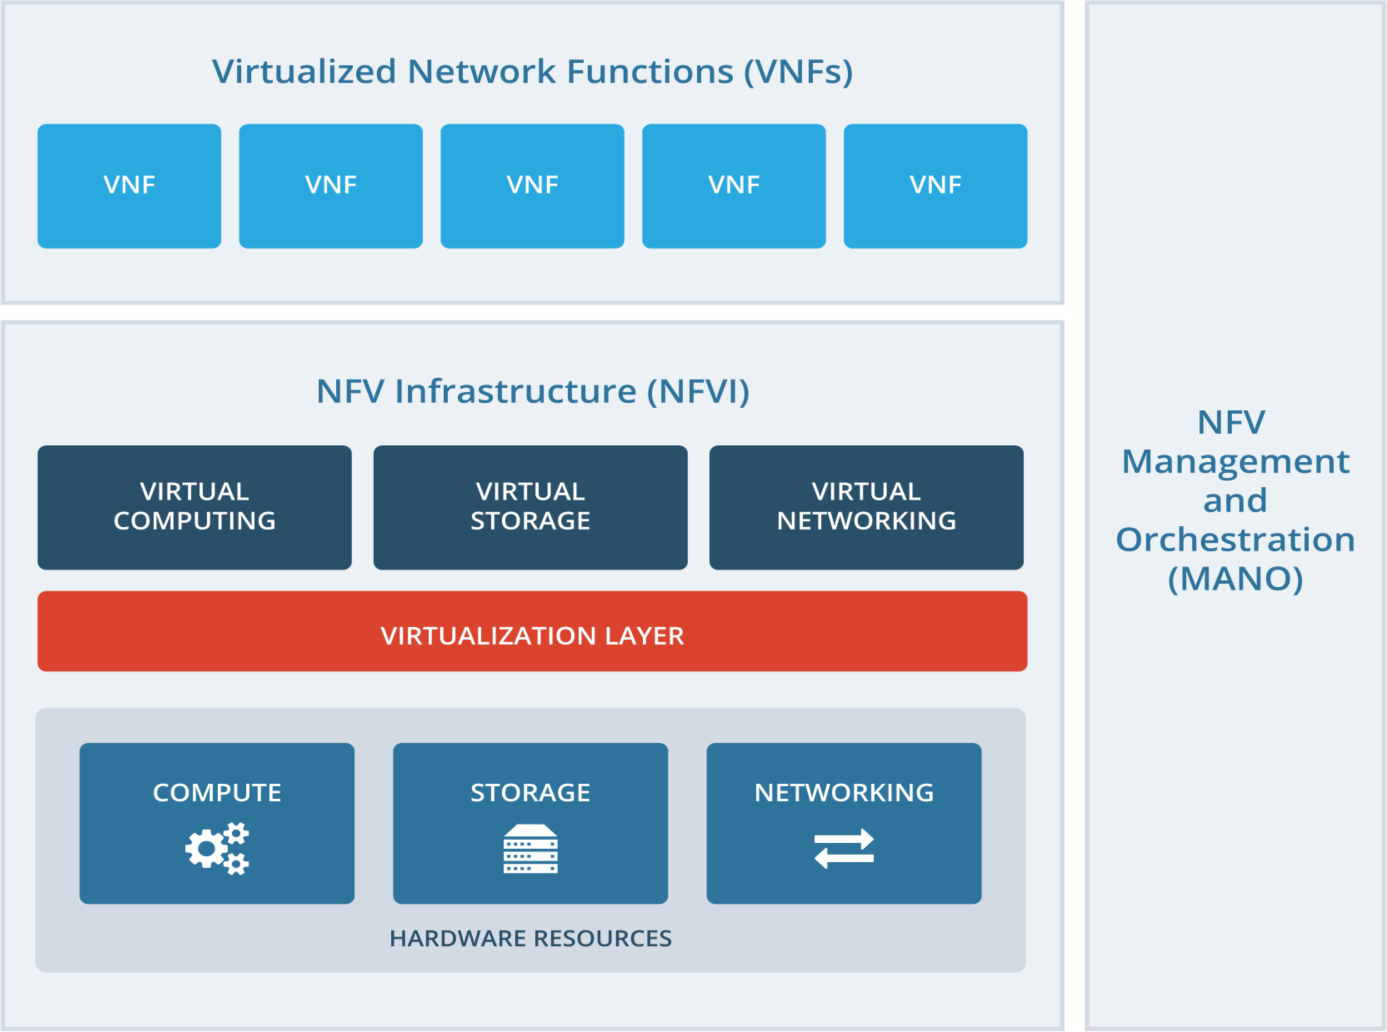
\includegraphics[width=1\linewidth]{OpenStackFoundationNFVReport}
		\caption{NFV functional overview\cite{openstack_nfv}}
		\label{fig:OpenStackFoundationNFVReport}
	\end{center}
	\vspace{-10pt}
\end{figure}

In an NFV environment, a virtual network function (VNF) takes on the responsibility of handling specific network functions that run on one or more virtual machines (VMs), on bare metal, or in containers, on top of the physical networking infrastructure.
A VNF can be an instance of any virtual hardware, for example: message router, CDN, DPI, Firewall, DNS...

The benefits of NFV stem from the fact that it runs on general purpose servers and switches in virtual machines or containers and is built with standard open APIs.

There are many ongoing NFV implementations. To keep it short, two of the NFV projects will be discussed.
\begin{itemize}
	\item Open Baton
	\item Tacker
\end{itemize}

\section{Open Baton - NFV Orchestrator}\label{sec:openbaton}
Open Baton is an European Telecommunications Standards Institute's (ETSI) NFV compliant Management and Orchestration (MANO) Framework.
It enables virtual Network Services deployments on top of the NFV infrastructure.

\begin{figure}[H]
	\begin{center}
		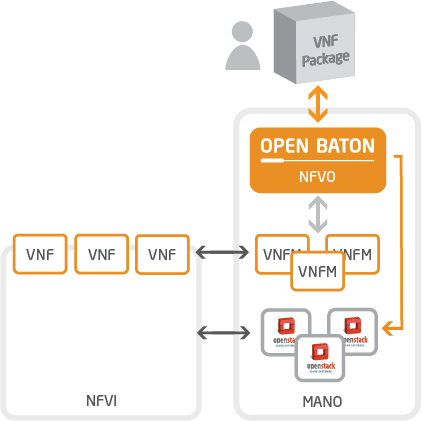
\includegraphics[width=1\linewidth]{openbaton_openstack}
		\caption{Placement of VNFM and VNF over the OpenStack Vitual Machines\cite{openBatonFeatures}}
		\label{fig:openbaton_openstack}
	\end{center}
	\vspace{-10pt}
\end{figure}

The Open Baton software is deployed over OpenStack with its own dashboard which would provide an easy to use web based VNF management console.
The VNF is configured on the virtual machine in the OpenStack IaaS.


\section{Tacker - OpenStack NFV Orchestration}\label{sec:tacker}

Tacker is an official OpenStack project building a Generic VNF Manager (VNFM) and a NFV Orchestrator (NFVO) to deploy and operate Network Services and Virtual Network Functions (VNFs) on an NFV infrastructure platform like OpenStack. It is based on ETSI MANO Architectural Framework and provides a functional stack to Orchestrate Network Services end-to-end using VNFs.


	% !TEX root       = ./type_name.tex
% !TEX program    = pdflatex
% !TEX encoding   = utf-8
% !TEX spellcheck = de_DE_frami
%=======================================================================

\chapter{Conclusion}\label{ch:Conclusion}

OpenStack is an emerging and stable open source Cloud Infrastructure-as-a-Service operating solution.
OpenStack, with it's usage as Compute service- to create cloud based computing or Storage service- for cloud based storage solutions or both combined, is an easily deployable cloud operating solution with minimum infrastructure to start hosting the Cloud service.

As this thesis is focussed on scheduling algorithm of requested virtual instances, it can be observed from the logs in Appendix \ref{app:sec:filterschedulerlogtrace10vi} that, with the standard nova FilterScheduler, when a large number of virtual instance creation is requested, it iterates for that number of times to provide a placement decision one after the another. There is an opportunity for improvement to solve a large requests with minimum time and better mathematical modelling.

In the section \nameref{sec:comparision} of the chapter \nameref{ch:comparisionofbothscheduler}, it can be observed that the cPlex based scheduling algorithm is effective in providing a placement decision which would reduce the operating power expense of the OpenStack cloud cluster by minimising the active(powered on) number of hosts.

This is also effective in timely creation of large quantity of virtual instances compared to the existing standard nova scheduler.

This thesis is an approach to have a different possible solution in the scheduling algorithm which could be helpful to have constraint dependant scheduling.

This thesis can also be extended to have two different scheduling solutions depending on the number of requests for creation of the virtual instances.
With a condition based on quantity of instance creation, the selection of the scheduler driver can be switched at runtime.

If the "Live Migration" could work effectively, the scheduling algorithm could also include the migration of existing instances to re-arrange itself which would increase the available capacity on the hosts and place new instances with larger configuration requirements.
This could also be helpful for live migration of multiple virtual instances when the compute nodes needs a maintenance downtime.

The cloud computing is the growing field of interest which creates lots of opportunities for research and as well as the ideas for business.
	
	%======================================================================
	%:Literaturverzeichnis
	%======================================================================
	\newpage
	\bibliographystyle{unsrtnat}
	\bibliography{bib/literatur}
	
	
	%======================================================================
	%:Anhang (TODO)
	%======================================================================
	\appendix
	\phantomsection{}
	\addcontentsline{toc}{chapter}{\appendixname}
	\addpart*{\appendixname}\label{p:anhang}
	
	% !TEX root       = ./type_name.tex
% !TEX program    = pdflatex
% !TEX encoding   = utf-8
% !TEX spellcheck = de_DE_frami
%=======================================================================

\chapter{Router Configuration Content}\label{app:ch:Routerconfig}

In this Appendix \nameref{app:ch:Routerconfig}, the reader can find the specifically mentioned configuration for the router.

\section{Wireless configuration}\label{app:sec:wireless_config}
The Wireless configuration parameters set in the \verb|[OpenWrt]| are:
\begin{lstlisting}[frame=single]
config wifi-device 'radio0'
option type 'mac80211'
option channel '11'
option hwmode '11g'
option path 'platform/ar934x_wmac'
option htmode 'HT20'
option txpower '20'
option country 'DE'
option disabled '0'

config wifi-iface
option device 'radio0'
option mode 'ap'
option ssid 'OpenWrt'
option server '192.168.1.169'
option key 'testing123'
option encryption 'wpa2'
option network 'wifi'

config wifi-device 'radio1'
option type 'mac80211'
option channel '36'
option hwmode '11a'
option path 'pci0000:00/0000:00:00.0'
option htmode 'HT20'
option txpower '17'
option country 'DE'

config wifi-iface
option device 'radio1'
option mode 'ap'
option server '192.168.1.169'
option key 'testing123'
option ssid 'OpenWrt 5G'
option encryption 'wpa2'
option network 'wifi'
\end{lstlisting}
\section{Network configuration}\label{app:sec:Network_config}
The Network configuration parameters set in the \verb|[OpenWrt]| are:
\begin{lstlisting}[frame=single]
config interface 'loopback'
option ifname 'lo'
option proto 'static'
option ipaddr '127.0.0.1'
option netmask '255.0.0.0'

config globals 'globals'
option ula_prefix 'fd04:beb4:615d::/48'

config interface 'wan'
option ifname 'eth0.1'
option proto 'dhcp'

config interface 'wan6'
option ifname 'eth0.1'
option proto 'dhcpv6'

config interface 'lan'
option type 'bridge'
option ifname 'eth0.2'
option proto 'static'
option ipaddr '192.168.1.1'
option netmask '255.255.255.0'
option ip6assign '60'

config interface 'wifi'
option type 'bridge'
option ifname 'eth0.3'
option proto 'static'
option ipaddr '192.168.3.1'
option netmask '255.255.255.0'
option ip6assign '60'

config interface 'lan3'
option ifname 'eth0.3'

config interface 'lan4'
option ifname 'eth0.4'

config interface 'lan5'
option ifname 'eth0.5'

config switch
option name 'switch0'
option reset '1'
option enable_vlan '1'

config switch_vlan
option device 'switch0'
option vlan '1'
option ports '1 0t'
option vid '1'

config switch_vlan
option device 'switch0'
option vlan '2'
option ports '2 0t'
option ipaddr '192.168.3.1'
option netmask '255.255.255.0'
option ip6assign '60'

config interface 'lan3'
option ifname 'eth0.3'

config interface 'lan4'
option ifname 'eth0.4'

config interface 'lan5'
option ifname 'eth0.5'

config switch
option name 'switch0'
option reset '1'
option enable_vlan '1'

config switch_vlan
option device 'switch0'
option vlan '1'
option ports '1 0t'
option vid '1'

config switch_vlan
option device 'switch0'
option vlan '2'
option ports '2 0t'
option vid '2'

config switch_vlan
option device 'switch0'
option vlan '3'
option ports '3 0t'
option vid '3'

config switch_vlan
option device 'switch0'
option vlan '4'
option vid '4'
option ports '0t 4'

config switch_vlan
option device 'switch0'
option vlan '5'
option vid '5'
option ports '0t 5'
\end{lstlisting}
\section{DHCP configuration}\label{app:sec:DHCP_config}
The DHCP configuration parameters set in the \verb|[OpenWrt]| are:
\begin{lstlisting}[frame=single]

config dnsmasq
option domainneeded '1'
option boguspriv '1'
option filterwin2k '0'
option localise_queries '1'
option rebind_protection '1'
option rebind_localhost '1'
option local '/lan/'
option domain 'lan'
option expandhosts '1'
option nonegcache '0'
option authoritative '1'
option readethers '1'
option leasefile '/tmp/dhcp.leases'
option resolvfile '/tmp/resolv.conf.auto'
option localservice '1'

config dhcp 'lan'
option interface 'lan'
option start '100'
option limit '150'
option leasetime '12h'
option dhcpv6 'server'
option ra 'server'

config dhcp 'wifi'
option interface 'wifi'
option start '100'
option limit '150'
option leasetime '12h'
option dhcpv6 'server'
option ra 'server'

config dhcp 'wan'
option interface 'wan'
option ignore '1'

config odhcpd 'odhcpd'
option maindhcp '0'
option leasefile '/tmp/hosts/odhcpd'
option leasetrigger '/usr/sbin/odhcpd-update'

config dhcp 'lan4'
option interface 'lan4'
option ignore '1'


\end{lstlisting}

\chapter{RYU Verbose output}\label{app:ch:logs}

In this Appendix, the logs from the \verb|/tmp/log| file have been provided for different log purpose.

\section{RYU log trace}\label{app:sec:RYUlogtrace}

\begin{lstlisting}[frame=single, caption={The RYU Verbose log}, label={lst:RYUverboselog}]
loading app usr_seg.py
loading app ryu.controller.ofp_handler
instantiating app usr_seg.py of SimpleSwitch13
instantiating app ryu.controller.ofp_handler of OFPHandler
BRICK SimpleSwitch13
CONSUMES EventOFPPacketIn
CONSUMES EventOFPSwitchFeatures
BRICK ofp_event
PROVIDES EventOFPPacketIn TO {'SimpleSwitch13': set(['main'])}
PROVIDES EventOFPSwitchFeatures TO {'SimpleSwitch13': set(['config'])}
CONSUMES EventOFPEchoRequest
CONSUMES EventOFPPortStatus
CONSUMES EventOFPEchoReply
CONSUMES EventOFPSwitchFeatures
CONSUMES EventOFPPortDescStatsReply
CONSUMES EventOFPHello
CONSUMES EventOFPErrorMsg
connected socket:<eventlet.greenio.base.GreenSocket object at 0x7f42b40851d0> address:('192.168.1.1', 58461)
hello ev <ryu.controller.ofp_event.EventOFPHello object at 0x7f42b4085a90>
move onto config mode
EVENT ofp_event->SimpleSwitch13 EventOFPSwitchFeatures
switch features ev version=0x4,msg_type=0x6,msg_len=0x20,xid=0xf35c1db1,OFPSwitchFeatures(auxiliary_id=0,capabilities=79,datapath_id=176968783353910,n_buffers=256,n_tables=254)
move onto main mode
EVENT ofp_event->SimpleSwitch13 EventOFPPacketIn
packet truncated: only 170 of 342 bytes
Timestamp 2017-02-16 12:49:36.274578
Timestamp 2017-02-16 12:49:36.276005
outport_for_src tuple is None
Data is 00:26:9e:e2:b2:f8
packet in 176968783353910 00:26:9e:e2:b2:f8 ff:ff:ff:ff:ff:ff 2
DST is ff:ff:ff:ff:ff:ff
Out_Port before else flood condition None
Out_Port is Flooded 4294967291
Above actions Out_Port 4294967291
Actions is [OFPActionOutput(len=16,max_len=65509,port=4294967291,type=0)]
EVENT ofp_event->SimpleSwitch13 EventOFPPacketIn
EVENT ofp_event->SimpleSwitch13 EventOFPPacketIn
EVENT ofp_event->SimpleSwitch13 EventOFPPacketIn
EVENT ofp_event->SimpleSwitch13 EventOFPPacketIn
EVENT ofp_event->SimpleSwitch13 EventOFPPacketIn
EVENT ofp_event->SimpleSwitch13 EventOFPPacketIn
EVENT ofp_event->SimpleSwitch13 EventOFPPacketIn
EVENT ofp_event->SimpleSwitch13 EventOFPPacketIn
EVENT ofp_event->SimpleSwitch13 EventOFPPacketIn
Timestamp 2017-02-16 12:49:36.485248
Timestamp 2017-02-16 12:49:36.486536
outport_for_src tuple is None
Data is 00:26:9e:e2:b2:f8
packet in 176968783353910 00:26:9e:e2:b2:f8 ff:ff:ff:ff:ff:ff 2
DST is ff:ff:ff:ff:ff:ff
Out_Port before else flood condition None
Out_Port is Flooded 4294967291
Above actions Out_Port 4294967291
Actions is [OFPActionOutput(len=16,max_len=65509,port=4294967291,type=0)]
Timestamp 2017-02-16 12:49:36.490576
Timestamp 2017-02-16 12:49:36.491804
outport_for_src tuple is None
Data is 00:26:9e:e2:b2:f8
packet in 176968783353910 00:26:9e:e2:b2:f8 33:33:ff:a2:39:fe 2
DST is 33:33:ff:a2:39:fe
Out_Port before else flood condition None
Out_Port is Flooded 4294967291
Above actions Out_Port 4294967291
Actions is [OFPActionOutput(len=16,max_len=65509,port=4294967291,type=0)]
Timestamp 2017-02-16 12:49:36.495438
Timestamp 2017-02-16 12:49:36.496494
outport_for_src tuple is None
Data is 00:26:9e:e2:b2:f8
packet in 176968783353910 00:26:9e:e2:b2:f8 33:33:ff:00:07:5c 2
DST is 33:33:ff:00:07:5c
Out_Port before else flood condition None
Out_Port is Flooded 4294967291
Above actions Out_Port 4294967291
Actions is [OFPActionOutput(len=16,max_len=65509,port=4294967291,type=0)]
Timestamp 2017-02-16 12:49:36.499691
Timestamp 2017-02-16 12:49:36.500575
outport_for_src tuple is None
Data is a0:0b:ba:c9:9e:04
packet in 176968783353910 a0:0b:ba:c9:9e:04 ff:ff:ff:ff:ff:ff 1
DST is ff:ff:ff:ff:ff:ff
Out_Port before else flood condition None
Out_Port is Flooded 4294967291
Above actions Out_Port 4294967291
Actions is [OFPActionOutput(len=16,max_len=65509,port=4294967291,type=0)]
EVENT ofp_event->SimpleSwitch13 EventOFPPacketIn
packet truncated: only 170 of 350 bytes
Timestamp 2017-02-16 12:52:47.115680
Timestamp 2017-02-16 12:52:47.116894
outport_for_src tuple is ('2',)
Data is a0:0b:ba:c9:9e:04
packet in 176968783353910 a0:0b:ba:c9:9e:04 ff:ff:ff:ff:ff:ff 1
DST is ff:ff:ff:ff:ff:ff
Out_Port before else flood condition ('2',)
Setting Out_Port same as in table, changing flow 2
Above actions Out_Port 2
Actions is [OFPActionOutput(len=16,max_len=65509,port=2,type=0)]
Out_Port not flooded adding flow 
EVENT ofp_event->SimpleSwitch13 EventOFPPacketIn
Data is c8:5b:76:1b:ed:41
packet in 176968783353910 c8:5b:76:1b:ed:41 ff:ff:ff:ff:ff:ff 3
DST is ff:ff:ff:ff:ff:ff
Out_Port before else flood condition None
Out_Port is Flooded 4294967291
Above actions Out_Port 4294967291
Actions is [OFPActionOutput(len=16,max_len=65509,port=4294967291,type=0)]
Timestamp 2017-02-16 12:53:03.276915
Timestamp 2017-02-16 12:53:03.277904
outport_for_src tuple is None
Data is c8:5b:76:1b:ed:41
packet in 176968783353910 c8:5b:76:1b:ed:41 33:33:00:01:00:03 3
DST is 33:33:00:01:00:03
Out_Port before else flood condition None
Out_Port is Flooded 4294967291
Above actions Out_Port 4294967291
Actions is [OFPActionOutput(len=16,max_len=65509,port=4294967291,type=0)]
Timestamp 2017-02-16 12:53:03.282229
Timestamp 2017-02-16 12:53:03.283229
outport_for_src tuple is None
Data is c8:5b:76:1b:ed:41
packet in 176968783353910 c8:5b:76:1b:ed:41 01:00:5e:00:00:fb 3
DST is 01:00:5e:00:00:fb
Out_Port before else flood condition None
Out_Port is Flooded 4294967291
Above actions Out_Port 4294967291
Actions is [OFPActionOutput(len=16,max_len=65509,port=4294967291,type=0)]
EVENT ofp_event->SimpleSwitch13 EventOFPPacketIn
Timestamp 2017-02-16 12:54:32.618185
Timestamp 2017-02-16 12:54:32.619362
outport_for_src tuple is ('3',)
Data is c0:ee:fb:20:41:24
packet in 176968783353910 c0:ee:fb:20:41:24 01:00:5e:00:00:16 1
DST is 01:00:5e:00:00:16
Out_Port before else flood condition ('3',)
Setting Out_Port same as in table, changing flow 3
Above actions Out_Port 3
Actions is [OFPActionOutput(len=16,max_len=65509,port=3,type=0)]
Out_Port not flooded adding flow 
EVENT ofp_event->SimpleSwitch13 EventOFPPacketIn
Timestamp 2017-02-16 12:54:36.051777
Timestamp 2017-02-16 12:54:36.052886
outport_for_src tuple is ('3',)
Data is c0:ee:fb:20:41:24
packet in 176968783353910 c0:ee:fb:20:41:24 01:00:5e:00:00:fb 1
DST is 01:00:5e:00:00:fb
Out_Port before else flood condition ('3',)
Setting Out_Port same as in table, changing flow 3
Above actions Out_Port 3
Actions is [OFPActionOutput(len=16,max_len=65509,port=3,type=0)]
Out_Port not flooded adding flow 
EVENT ofp_event->SimpleSwitch13 EventOFPPacketIn
Timestamp 2017-02-16 12:55:09.360397
Timestamp 2017-02-16 12:55:09.361360
\end{lstlisting}


	% !TEX root       = ./type_name.tex
% !TEX program    = pdflatex
% !TEX encoding   = utf-8
% !TEX spellcheck = de_DE_frami
%=======================================================================

\chapter{User Segregation Application code}\label{app:ch:app_code}

In this Appendix \nameref{app:ch:app_code}, the entire application code written in Python is listed here.


\begin{lstlisting}[language = Python, caption={The User Segregation Mac Learning Application}, label={lst:userseg-code}]
# Copyright (C) 2011 Nippon Telegraph and Telephone Corporation.
#
# Licensed under the Apache License, Version 2.0 (the "License");
# you may not use this file except in compliance with the License.
# You may obtain a copy of the License at
#
#    http://www.apache.org/licenses/LICENSE-2.0
#
# Unless required by applicable law or agreed to in writing, software
# distributed under the License is distributed on an "AS IS" BASIS,
# WITHOUT WARRANTIES OR CONDITIONS OF ANY KIND, either express or
# implied.
# See the License for the specific language governing permissions and
# limitations under the License.
import MySQLdb
import sys
import datetime
from ryu.base import app_manager
from ryu.controller import ofp_event
from ryu.controller.handler import CONFIG_DISPATCHER, MAIN_DISPATCHER
from ryu.controller.handler import set_ev_cls
from ryu.ofproto import ofproto_v1_3
from ryu.lib.packet import packet
from ryu.lib.packet import ethernet
from ryu.lib.packet import ether_types
from ryu.lib.packet import udp



class SimpleSwitch13(app_manager.RyuApp):
	OFP_VERSIONS = [ofproto_v1_3.OFP_VERSION]

	def __init__(self, *args, **kwargs):
		super(SimpleSwitch13, self).__init__(*args, **kwargs)
		self.mac_to_port = {}

	@set_ev_cls(ofp_event.EventOFPSwitchFeatures, CONFIG_DISPATCHER)
	def switch_features_handler(self, ev):
		datapath = ev.msg.datapath
		ofproto = datapath.ofproto
		parser = datapath.ofproto_parser

		# install table-miss flow entry
		#
		# We specify NO BUFFER to max_len of the output action due to
		# OVS bug. At this moment, if we specify a lesser number, e.g.,
		# 128, OVS will send Packet-In with invalid buffer_id and
		# truncated packet data. In that case, we cannot output packets
		# correctly.  The bug has been fixed in OVS v2.1.0.
		match = parser.OFPMatch()
		actions = [parser.OFPActionOutput(ofproto.OFPP_CONTROLLER, ofproto.OFPCML_NO_BUFFER)]
		self.add_flow(datapath, 0, match, actions)

	def add_flow(self, datapath, priority, match, actions, buffer_id=None):
		ofproto = datapath.ofproto
		parser = datapath.ofproto_parser

		inst = [parser.OFPInstructionActions(ofproto.OFPIT_APPLY_ACTIONS, actions)]
		if buffer_id: 
			mod = parser.OFPFlowMod(datapath=datapath, buffer_id=buffer_i , priority=priority, match=match, instructions=inst)
		else:
			mod = parser.OFPFlowMod(datapath=datapath, priority=priority, match=match, instructions=inst)
			
		datapath.send_msg(mod)

	@set_ev_cls(ofp_event.EventOFPPacketIn, MAIN_DISPATCHER)
	def _packet_in_handler(self, ev):
	# If you hit this you might want to increase
	# the "miss_send_length" of your switch

		if ev.msg.msg_len < ev.msg.total_len:
			self.logger.debug("packet truncated: only %s of %s bytes", ev.msg.msg_len, ev.msg.total_len)
		msg = ev.msg
		datapath = msg.datapath
		ofproto = datapath.ofproto
		parser = datapath.ofproto_parser
		in_port = msg.match['in_port']

		pkt = packet.Packet(msg.data)
		eth = pkt.get_protocols(ethernet.ethernet)[0]
		udp_payload = pkt.get_protocols(udp.udp)


		if eth.ethertype == ether_types.ETH_TYPE_LLDP:
			# ignore lldp packet
			return
		dst = eth.dst
		src = eth.src

		dpid = datapath.id
		self.mac_to_port.setdefault(dpid, {})
	

	#creating a mysql connection to database -last edit 17/11

	connection = MySQLdb.connect(host = "192.168.1.169", user = "freerad", passwd = "pass", db = "radius")
	cursor = connection.cursor ()
	cursor.execute ("SELECT portid FROM radcheck WHERE username IN (SELECT user FROM radpostauth WHERE CallingStationId = %s AND id = (SELECT MAX(id) from radpostauth) )", src)
	outport_for_src = cursor.fetchone ()

	cursor.close()
	connection.close ()
	# Mysql verification end


		# learn a mac address to avoid FLOOD next time.
		self.mac_to_port[dpid][src] = in_port
	
	if dst in self.mac_to_port[dpid]:
		test = self.mac_to_port[dpid][dst]
		
		if outport_for_src != None and all(outport_for_src):
			if int(outport_for_src[0]) == self.mac_to_port[dpid][dst]:
				out_port = self.mac_to_port[dpid][dst]

			else:

				return

		else:
		#except (TypeError,UnboundLocalError):		
			out_port = self.mac_to_port[dpid][dst]		

	else:

		if outport_for_src != None and all(outport_for_src): out_port = int(outport_for_src[0])

		else:
		#except (TypeError,UnboundLocalError):

			out_port = ofproto.OFPP_FLOOD

		actions = [parser.OFPActionOutput(out_port)]


		# install a flow to avoid packet_in next time
		if out_port != ofproto.OFPP_FLOOD:

			match = parser.OFPMatch(in_port=in_port, eth_dst=dst)
			#match = parser.OFPMatch(in_port=in_port, eth_dst='a0:f3:c1:77:d8:36')
			# verify if we have a valid buffer_id, if yes avoid to send both
			# flow_mod & packet_out
			if msg.buffer_id != ofproto.OFP_NO_BUFFER:
				self.add_flow(datapath, 1, match, actions, msg.buffer_id)
				return
			else:
				self.add_flow(datapath, 1, match, actions)
		data = None

		if msg.buffer_id == ofproto.OFP_NO_BUFFER:
			data = msg.data

		out = parser.OFPPacketOut(datapath=datapath, buffer_id=msg.buffer_id, in_port=in_port, actions=actions, data=data)
		datapath.send_msg(out)

\end{lstlisting}


	
	
	
	
	%======================================================================
	%:Selbstständigkeitserklärung
	%======================================================================
	\addchap{Versicherung}
	
	Hiermit versichere ich, dass ich die vorliegende Arbeit ohne unzulässige Hilfe Dritter und ohne
	Benutzung anderer als der angegebenen Hilfsmittel angefertigt habe; die aus fremden Quellen direkt
	oder indirekt übernommenen Gedanken sind als solche kenntlich gemacht.\\
	Bei der Auswahl und Auswertung des Materials sowie bei der Herstellung des Manuskripts habe ich
	Unterstützungsleistungen von folgenden Personen erhalten: \\[2ex]
	\hspace*{\fill}keine\hspace*{\fill}\\[2ex]
	Weitere Personen waren an der Abfassung der vorliegenden Arbeit nicht beteiligt. Die Hilfe eines
	Promotionsberaters habe ich nicht in Anspruch genommen. Weitere Personen haben von mir keine
	geldwerten Leistungen für Arbeiten erhalten, die im Zusammenhang mit dem Inhalt der vorgelegten
	Dissertation stehen.
	
	Die Arbeit wurde bisher weder im Inland noch im Ausland in gleicher oder ähnlicher Form einer
	anderen Prüfungsbehörde vorgelegt.
	
	\vspace{4ex}
	\begin{flushleft}
		\dcplace, \dcdate\\[8ex]
		\newlength\us\settowidth{\us}{-\dcauthorfirstname~\dcauthorlastname-}
		\begin{tabular}{p{\us}}\midrule
			\centering\footnotesize \dcauthorfirstname~\dcauthorlastname{}
		\end{tabular}
	\end{flushleft}
	
\end{document}
%=======================================================================
% vim: ts=2:sw=2:sts=2:expandtab:wrapmargin=2:tw=120

